
\subsubsection{Documentazione interna}
La documentazione interna comprende tutti i documenti che contengono informazioni utili principalmente per il gruppo, e che vengono quindi consultati di conseguenza. 
\paragraph{\textit{Verbale}}
Il verbale ha lo scopo di rendicontare ciò che viene detto durante una riunione.
Rispetta la struttura generale.
In aggiunta presenta:
\begin{itemize} 
    \item \textbf{Informazioni Generali}
    contiene:
    \begin{itemize} 
        \item Luogo;
        \item Data;
        \item Ora;
        \item Partecipanti.
    \end{itemize}
\item \textbf{Tabella tracciamento temi affrontati}:
tabella che riassume i punti salienti della riunione indicandone:
    \begin{itemize} 
        \item Codice: ha il formato V\textbf{X} \textbf{Y}.\textbf{Z} dove X indica la tipologia di \textit{Verbale}, Y indica il numero di \textit{Verbale} (incrementale rispetto agli altri verbali);
        e Z indica il numero dell'argomento trattato (incrementale rispetto agli altri argomenti del \textit{Verbale});
        \item Descrizione: breve descrizione di uno specifico argomento trattato.
    \end{itemize}
\end{itemize}
\paragraph{\textit{Studio di Fattibilità}}
Lo \textit{Studio di Fattibilità} ha lo scopo di valutare i pro ed i contro dei capitolati proposti in modo da scegliere il più vantaggioso al quale candidarsi.
La scelta del capitolato viene fatta sulla base di diverse considerazioni.
Vengono valutati:
\begin{itemize}
    \item \textbf{Risorse}: in termini di budget, tempo e personale;
    \item \textbf{Previe Conoscenze}: un capitolato potrebbe rivelarsi più o meno difficile da realizzare a seconda delle conoscenze del contesto applicativo; 
    \item \textbf{Guadagno}: un capitolato potrebbe venire scartato per scarso guadagno netto al termine del lavoro commissionato (non è il nostro caso ma 
andrebbe tenuto in considerazione in ambito lavorativo);
    \item \textbf{Aspetti psicologici}: avendo la possibilità di scegliere tra capitolati (fatto che capita raramente in un reale ambito lavorativo) di pari interesse siamo portati a scegliere il contesto applicativo che ci entusiasma maggiormente.
    Questo aspetto potrebbe avere un impatto positivo sulla produttività del gruppo.
\end{itemize}

Il documento tiene in considerazione tutti i capitolati proposti per non scartare un capitolato per le sensazioni soggettive dei componenti del gruppo.
Non tenendo in considerazione ogni capitolato, infatti, si potrebbe scartare un capitolato di forte interesse senza rendersene conto.
\documentclass[a4paper]{article}
\usepackage[normalem]{ulem}

% impostazioni generali
%Tutti gli usepackage vanno qui
\usepackage{geometry}
\usepackage[italian]{babel}
\usepackage[utf8]{inputenc}
\usepackage{tabularx}
\usepackage{longtable}
\usepackage{hyperref}
\usepackage{enumitem}
\usepackage{array} 
\usepackage{booktabs}
\newcolumntype{M}[1]{>{\centering\arraybackslash}m{#1}}
\usepackage[toc]{appendix}

\hypersetup{
	colorlinks=true,
	linkcolor=blue,
	filecolor=magenta,
	urlcolor=blue,
}
% Numerazione figure
\let\counterwithout\relax
\let\counterwithin\relax
\usepackage{chngcntr}

% distanziare elenco delle figure e delle tabelle
\usepackage{tocbasic}
\DeclareTOCStyleEntry[numwidth=3.5em]{tocline}{figure}% for figure entries
\DeclareTOCStyleEntry[numwidth=3.5em]{tocline}{table}% for table entries


\counterwithin{table}{subsection}
\counterwithin{figure}{subsection}

\usepackage[bottom]{footmisc}
\usepackage{fancyhdr}
\setcounter{secnumdepth}{4}
\usepackage{amsmath, amssymb}
\usepackage{array}
\usepackage{graphicx}

\usepackage{ifthen}

\usepackage{float}
\restylefloat{table}

\usepackage{layouts}
\usepackage{url}
\usepackage{comment}
\usepackage{eurosym}

\usepackage{lastpage}
\usepackage{layouts}
\usepackage{eurosym}

\geometry{a4paper,top=3cm,bottom=4cm,left=2.5cm,right=2.5cm}

%Comandi di impaginazione uguale per tutti i documenti
\pagestyle{fancy}
\lhead{
\includegraphics[scale=0.1]{../../../template/images/logo_no_motto.jpeg}}
%Titolo del documento
\rhead{\doctitle{}}
%\rfoot{\thepage}
\cfoot{Pagina \thepage\ di \pageref{LastPage}}
\setlength{\headheight}{35pt}
\setcounter{tocdepth}{5}
\setcounter{secnumdepth}{5}
\renewcommand{\footrulewidth}{0.4pt}

% multirow per tabelle
\usepackage{multirow}

% Permette tabelle su più pagine
%\usepackage{longtable}


% colore di sfondo per le celle
\usepackage[table]{xcolor}

%COMANDI TABELLE
\newcommand{\rowcolorhead}{\rowcolor[HTML]{007c95}}
\newcommand{\cellcolorhead}{\cellcolor[HTML]{007c95}}
\newcommand{\hlinetable}{\arrayrulecolor[HTML]{007c95}\hline}

%intestazione
% check for missing commands
\newcommand{\headertitle}[1]{\textbf{\color{white}#1}} %titolo colonna
\definecolor{pari}{HTML}{b1dae3}
\definecolor{dispari}{HTML}{d7f2f7}

% comandi glossario
\newcommand{\glo}{$_{G}$}
\newcommand{\glosp}{$_{G}$ }


%label custom
\makeatletter
\newcommand{\uclabel}[2]{%
	\protected@write \@auxout {}{\string \newlabel {#1}{{#2}{\thepage}{#2}{#1}{}} }%
	\hypertarget{#1}{#2}
}
\makeatother

%riportare pezzi di codice
\definecolor{codegray}{gray}{0.9}
\newcommand{\code}[1]{\colorbox{codegray}{\texttt{#1}}}



% dati relativi alla prima pagina
% Configurazione della pagina iniziale
\newcommand{\doctitle}{\textit{Verbale} interno 01-12-2022 }
\newcommand{\docdate}{01 Dicembre 2022}
\newcommand{\rev}{1.0.0}
\newcommand{\stato}{Approvato}
\newcommand{\uso}{Interno}
\newcommand{\approv}{Elena Pandolfo}
\newcommand{\red}{Tommaso Allegretti}
\newcommand{\ver}{Gabriele Mantoan\\& Mirko Stella}
\newcommand{\dest}{\textit{Seven Clickers}
									  \\ Prof. Vardanega Tullio 
									   \\ Prof. Cardin Riccardo}
\newcommand{\describedoc}{\textit{Verbale} riguardante il meeting tenuto il giorno 01-12-2022}


 % editare questo

\makeindex

\begin{document}
\counterwithin{table}{section}

% Prima pagina
\thispagestyle{empty}
\renewcommand{\arraystretch}{1.3}

\begin{titlepage}
	\begin{center}
		
	
\includegraphics[scale = 0.40]{../../../template/images/logo.jpeg}
	\\[1cm]
	\href{mailto:7clickersgroup@gmail.com}		      	
	{\large{\textit{7clickersgroup@gmail.com} } }\\[2.5cm]
	\Huge \textbf{\doctitle} \\[1cm]
	 \large
			 \begin{tabular}{r|l}
                        \textbf{Versione} & \rev{} \\
                        \textbf{Stato} & \stato{} \\
                        \textbf{Uso} & \uso{} \\                         
                        \textbf{Approvazione} & \approv{} \\                      
                        \textbf{Redazione} & \red{} \\ 
                        \textbf{Verifica} &  \ver{} \\                         
                        \textbf{Distribuzione} & \parbox[t]{5cm}{ \dest{} }
                \end{tabular} 
                \\[3.5cm]
                \large \textbf{Descrizione} \\ \describedoc{} 
     \end{center}
\end{titlepage}

% Diario delle modifiche
\section*{Registro delle modifiche}

\newcommand{\changelogTable}[1]{
	 

\renewcommand{\arraystretch}{1.5}
\rowcolors{2}{pari}{dispari}
\begin{longtable}{ 
		>{\centering}M{0.07\textwidth} 
		>{\centering}M{0.13\textwidth}
		>{\centering}M{0.20\textwidth}
		>{\centering}M{0.17\textwidth} 
		>{\centering\arraybackslash}M{0.30\textwidth} 
		 }
	\rowcolorhead
	\headertitle{Vers.} &
	\centering \headertitle{Data} &	
	\headertitle{Autore} &
	\headertitle{Ruolo} & 
	\headertitle{Descrizione} 
	\endfirsthead	
	\endhead
	
	#1

\end{longtable}
\vspace{-2em}

}



\changelogTable{
	1.0.0 & 14-12-22 & Elena Pandolfo & Responsabile &  Approvazione documento\tabularnewline
	0.1.0 & 01-12-22 & Gabriele Mantoan \\ Mirko Stella & Verificatori & Verifica documento\tabularnewline
	0.0.1 & 09-11-22 & Rino Sincic & Analista &  Redazione documento\\
} % editare questo
\pagebreak

% Indice
{
    \hypersetup{linkcolor=black}
    \tableofcontents
}
\pagebreak

% Contenuto
\section{Introduzione}
\subsection{Scopo del documento}
Lo scopo del documento è quello di stabilire le regole che ogni componente del gruppo SevenClickers
deve rispettare per mantenere un ambiente di lavoro che mira a massimizzare
l'economicità dei processi durante il ciclo di vita del prodotto ShowRoom3D.\\
Le norme verranno inserite in modo incrementale per regolamentare le attività di progetto imminenti rimandando quelle meno urgenti a quando 
se ne presenterà la necessità.\\
Inoltre tali norme potranno subire modifiche nel tempo in modo da garantire un miglioramento continuo della qualità del lavoro svolto.
Il responsabile di progetto ha il compito di comunicare l'aggiunta di una nuova norma o la modifica di una già esistente a tutti i componenti
del gruppo e di assicurarsi che siano comprese a pieno.
\subsection{Scopo del prodotto}
Il prodotto in questione nasce dalla necessità dell'azienda SanMarco Informatica di fornire una soluzione agli sprechi
derivati dall'adozione di uno ShowRoom tradizionale proponendo uno ShowRoom3D che sia 
ugualmente o ancora più immersivo.
\pagebreak

\section{Documentazione}
Questa sezione descrive le convenzioni,gli strumenti e le modalità con cui il gruppo si impegna a stilare la documentazione interna ed esterna relativa al progetto.

\subsubsection{Convenzioni generali}
Le convenzioni di seguito riportate vengono applicate a tutti i documenti.
Esse rendono i documenti stilati omogenei tra loro contribuendo a rendere il progetto professionale.

\paragraph{Versionamento}
Il numero di versione permette di capire lo stato in cui si trova un documento.
Un documento può trovarsi nei seguenti stati:
\begin{itemize} 
    \item \textbf{Approvato}: il documento è verificato ed approvato dal Responsabile;
    \item \textbf{Verificato}: il documento risulta verificato ma non ancora visionato dal Responsabile;
    \item \textbf{In Sviluppo}: sono presenti delle modifiche che non sono state verificate.
\end{itemize}
Il numero di versione ha il formato \textbf{X.Y.Z} dove:
\begin{itemize} 
    \item \textbf{X}: indica una versione approvata dal Responsabile, la numerazione parte da 0
    e la prima versione approvata è la 1.0.0;
    \item \textbf{Y}: indica una versione verificata dal Verificatore, la numerazione inizia da 0 e si azzera ad ogni incremento di X. La prima versione
    verificata è la 0.1.0;
    \item \textbf{Z}: indica una versione in fase di modifica da parte dei redattori che ne incrementano il numero ad ogni modifica,
    la numerazione parte da 1 e si azzera ad ogni incremento di X o Y. La prima versione modificata è la 0.0.1.
\end{itemize}

\paragraph{Struttura Generale}
Ogni documento deve presentare le seguenti sezioni nell'ordine in cui vengono presentate:
\begin{itemize} 
    \item \textbf{Intestazione}:
    contiene:
    \begin{itemize} 
        \item Logo compreso di motto;
        \item Indirizzo email di gruppo; 
        \item Titolo;
        \item Tabella contenente le informazioni generali:
        \begin{itemize}
            \item Versione;
            \item Stato;
            \item Uso;
            \item Approvazione: indica il responsabile di progetto che ha approvato il documento; 
            \item Redazione: elenco dei collaboratori che hanno partecipato alla stesura del documento;
            \item Verifica: elenco dei verificatori che hanno verificato il documento;
            \item Distribuzione: elenco delle persone o organizzazioni a cui è destinato il documento.
        \end{itemize}
        \item Breve descrizione del documento .
    \end{itemize}
    \item \textbf{Registro delle modifiche}:
    tabella che identifica ogni versione del documento indicandone:
    \begin{itemize} 
        \item Versione;
        \item Data;
        \item Autore;
        \item Ruolo;
        \item Descrizione.
    \end{itemize}
    \item \textbf{Indice}:
    elenco ordinato dei titoli dei capitoli, ovvero delle varie parti di cui si compone il documento;
    \item \textbf{Contenuto}:
    varia a seconda del tipo di documento.
\end{itemize}
\paragraph{Date}
Le date devono rispettare il seguente formato: \textbf{dd-mm-yyyy}
All'interno delle tabelle il formato deve essere il seguente: \textbf{dd-mm-yy}
\paragraph{Nomi di persona}
All'interno dei documenti i nomi di persona rispetteranno l'ordine nome seguito dal cognome della persona menzionata.

\paragraph{Elenchi puntati}
Gli elenchi puntati devono rispettare le seguenti regole:
\begin{itemize} 
    \item Ogni elemento dell'elenco deve iniziare con la lettera maiuscola;
    \item Ogni elemento dell'elenco deve terminare con ";" ad eccezione dell'ultimo elemento
    che deve terminare con "."; 
    \item Dopo i due punti la frase deve iniziare con la lettera minuscola.
\end{itemize}

\paragraph{Stile del testo}
\begin{itemize} 
    \item \textbf{Grassetto}: stile utilizzato per i titoli delle sezioni e per i primi termini degli elenchi puntati;
    \item \textbf{Corsivo}: viene utilizzato per citare il nome dei documenti, ad esempio \textit{Piano di Progetto}. 
\end{itemize}

\subsection{Verifica}
La verifica viene svolta da due verificatori prima del merge con il branch documentation.
Consiste nell'esaminare i file prodotti da chi ne ha fatto la stesura e segnalarne la non validità o 
la presenza di errori nei concetti esposti.\\
Un verificatore dovrà verificare il documento a partire dalle modifiche fatte dopo l'ultima versione verificata.
Le modifiche da verificare quindi possono essere dedotte dal registro dei cambiamenti presente in ogni documento.
Una volta controllato il documento, il primo verificatore segnalerà eventuali errori e
successivamente dovrà spuntare come approvata la Pull Request nella sezione dedicata su GitHub\textsubscript{g}. \\
A questo punto se un secondo verificatore noterà la necessità di qualche altro cambiamento da apportare, chi dovrà apportare le modifiche farà una pull in locale per
allineare il proprio branch con quello in remoto e continuare con il proprio lavoro.\\
Dopo il push delle modifiche se i file risultano corretti anche dal secondo verificatore esso aggiungerà i nomi dei verificatori all'intestazione modificando il file titlepage\_input.tex
 e creerà la riga nel registro delle modifiche, nel file changelog\_input.tex,  inserendo la nuova versione secondo le regole di versionamento e scrivendo nella colonna Autore sia il suo nome,
che quello del primo verificatore, e in descrizione "Verifica".
Dopo aver eseguito un commit sul ramo da integrare approva la Pull Request e conferma il merge secondo le norme di progetto descritte nella sezione dedicata.
\subsection{Approvazione}
L’approvazione viene svolta dal Responsabile di Progetto.\\
L'approvazione consiste nell'aprire una Pull Request di approvazione. Nel caso in cui il Responsabile di progetto riscontrasse ulteriori problematiche, segnalerà ai Verificatori le eventuali modifiche da apportare. I verificatori apporteranno tali modifiche prima di chiudere la Pull Request di approvazione e quindi di integrare i cambiamenti nel branch documentation.\\
Per i verbali si effettua questa pratica non appena il file prodotto viene verificato e quindi passa tutte le eventuali reviews create dai verificatori mentre per tutti gli altri documenti prima di una consegna.\\
Ad esito positivo di approvazione, il Responsabile di Progetto creerà una nuova riga e compilerà i campi nelle colonne corrispondenti del registro delle modifiche inserendo: l'ultima versione secondo le norme di versionamento, la data, il proprio nome, il suo ruolo e la voce "Approvazione" nell'ultima colonna.
\subsubsection{Strumenti per la stesura}
\begin{itemize} 
    \item LaTeX: è un linguaggio di marcatura per la preparazione di testi, basato sul 				  		  programma di composizione tipografica TEX.\\
	Nel branch documentation  si possono trovare i file .pdf prodotti e la cartella “latex”. La cartella latex contiene tre cartelle interne:
	\begin{itemize}
	\item esterni e interni, contengono file .tex di documentazione esterna ed interna come ad esempio i verbali o altra documentazione esterna/interna:
	\begin{itemize}
		\item la cartella config, contiene i file .tex con le parti fisse dei documenti (intestazione,registro delle modifiche,tracciamento dei temi affrontati) che vengono modificati con i dati del documento specifico 
		\item la cartella res/sections, contiene i file .tex con il contenuto vero e proprio (sezioni del documento) che viene redatto in maniera libera dal redattore
		\item un file col nome del documento pdf con estensione .tex che viene compilato per produrre il file pdf
	\end{itemize}
	 \item template, contiene file .tex di base utilizzati secondo necessità per comporre i documenti:
	 \begin{itemize}
	 \item changelox.tex è il file di template che serve per scrivere il registro delle modifiche
	 \item package.tex è il file che contiene tutti gli usepackage\textsubscript{g}
	 \item titlepage.tex è il file di template che contiene la configurazione della pagina iniziale di ogni documento  
	 \item tracking.tex è il file di template che contiene il tracciamento dei temi affrontati nel documento
	 \end{itemize}
	\end{itemize}
\end{itemize}

\pagebreak
\section{Strumenti collaborativi}
\subsection{GitHub\textsubscript{g}}
Servizio di hosting per progetti software che implementa uno strumento di controllo versione distribuito Git\textsubscript{g}.
Oltre alla copia in remoto del repository\textsubscript{g} di progetto ogni componente del gruppo ha una propria copia in locale.\\
Per ottenere una copia del repository\textsubscript{g} ogni componente ha scaricato lo strumento Git\textsubscript{g} ed eseguendo il 
comando 'git clone' da git\textsubscript{g} bash viene creata una cartella collegata alla repository\textsubscript{g} di progetto.\\
Non sono state imposte modalità specifiche sull'interazione con il repository\textsubscript{g} remoto in modo da non sconvolgere le abitudini di lavoro di 
ciascun componente.\\
I componenti del gruppo abituati ad interagire con GitHub\textsubscript{g} da interfaccia grafica possono continuare a farne uso.
\subsubsection{Repository\textsubscript{g}}
Il repository\textsubscript{g} si può trovare all'indirizzo \textbf{\textit{https://github.com/7clickers/ShowRoom3D}} ed è pubblico. 
I collaboratori sono i componenti del gruppo SevenClickers che utilizzano il proprio account GitHub\textsubscript{g} personale per collaborare al progetto.
\subsubsection{Branching}
\textbf{Branches protetti}:
    \begin{itemize} 
        \item main: contiene le versioni di release\textsubscript{g} del software
        \item documentation: contiene i template latex\textsubscript{g} e rispettivi pdf della documentazione
    \end{itemize}
\textit{documentation}: 
I documenti presenti in documentation sono stati approvati dal Responsabile di progetto o almeno verificati dai verificatori.\\
Per integrare delle modifiche da un branch protetto ad uno libero si utilizza un branch d’appoggio creato in locale partendo dall'ultimo commit di documentation e facendone il merge con il branch che necessita delle integrazioni. In seguito il branch di appoggio verrà eliminato.\\
\textbf{Branches liberi}:
Vengono utilizzati per creare nuove funzionalità e gli sviluppatori possono effettuare i commit senza l'approvazione degli altri componenti del gruppo
in quanto ciascun componente sviluppa su un solo branch alla volta salvo casi eccezionali.
Un branch\textsubscript{g} libero avrà il nome del documento che si sviluppa su quel branch\textsubscript{g}, oppure della feature\textsubscript{g} che va ad implementare.\\
Non appena i/il file nel branch sono stati verificati ed il merge è stato fatto, il branch libero verrà eliminato.
I branch di approvazione saranno chiamati con la sintassi appr\_nomefile1\_nomefile2\_nomefile3.... a seconda dei file che verranno approvati durante il ciclo di vita del branch.
\subsubsection{Commits}
È preferibile che ogni commit abbia una singola responsabilità per cambiamento.\\
I commits non possono essere effettuati direttamente sui branch protetti ma per integrare delle aggiunte o modifiche sarà necessario aprire una Pull Request.
All'approvazione di una Pull Request tutti i commit relativi al merge verranno raggruppati in un unico commit che rispetti la struttura sintattica descritta in seguito.

I commit dovranno essere accompagnati da una descrizione solo se ritenuta indispensabile alla comprensione del commit stesso.

I messaggi di commit sui \textbf{\uppercase{branch protetti}} dovranno seguire la seguente struttura sintattica:\\

\textbf{$<$label$>$$<$\#n\_issue$>$$<$testo$>$}\\\\
dove:\\\\
\textbf{label}: può assumere i seguenti valori
\begin{itemize}
\item feat: indica che è stata implementata una nuova funzionalità
\item fix: indica che è stato risolto un bug
\item update: indica che è stata apportata una modifica che non sia fix o feat
\item test: qualsiasi cosa legata ai test
\item docs: qualsiasi cosa legata alla documentazione
\end{itemize}
\textbf{n\_issue}: indica il numero della issue a cui fa riferimento il commit (se non fa riferimento a nessuna issue viene omesso).\\\\
\textbf{testo}:indica con quale branch è stato effettuato il merge e deve rispettare la forma: merge from $<$nome branch da integrare$>$ to $<$nome branch corrente$>$ \\\\
\textbf{descrizione}: se aggiunta ad un commit deve rispondere alle domande WHAT?,WHY?,HOW? ovvero
cosa è cambiato,perchè sono stati fatti i cambiamenti,in che modo sono stati fatti i cambiamenti.\\

I messaggi di commit sui \textbf{\uppercase{branch liberi}} dovranno seguire la struttura sintattica dei branch protetti ad eccezione del testo.
Il testo dei commit sui branch liberi non è soggetto a restrizioni particolari a patto che indichi in maniera intuitiva i cambiamenti fatti
in modo che possano essere compresi anche dagli altri collaboratori.



\subsubsection{Pull Requests}
Per effettuare un merge su un branch protetto si deve aprire da GitHub\textsubscript{g} una Pull Request.
La Pull Request permette di verificare il lavoro svolto prima di integrarlo con il branch desiderato.\\
Alla creazione di una Pull Request bisogna associare:
\begin{itemize}
\item i verificatori in carica hanno il compito di trovare eventuali errori o mancanze e fornire un feedback riguardante il contenuto direttamente su GitHub\textsubscript{g} richiedendo
una review con un review comment sulla parte specifica da revisionare o con un commento generico.\\
Non sarà possibile effettuare il merge finchè tutti i commenti di revisione non saranno stati risolti e la Pull Request approvata da due verificatori
\item l’issue associata nell’opzione “Development” che verrà chiusa alla risoluzione della Pull Request
\item la Projects Board di cui fa parte
\item gli assegnatari che hanno il compito di apportare le modifiche necessarie in fase di verifica
\item le labels associate
\end{itemize}
Per i commit relativi alle Pull Requests seguire le regole descritte nella sottosezione Commits per i branch protetti.

\subsubsection{Milestone\textsubscript{g}}
Una milestone indica un traguardo intermedio significativo per il progetto.
Ad essa possono venire assegnate delle issues per verificarne il raggiungimento.
Ogni milestone ha una scadenza che viene discussa e fissata da tutto il gruppo.
Oltre alle 2 milestone + 1 milestone falcoltativa fissate dal committente il gruppo ne creerá ulteriori per scandire piú nel dettaglio i passi che ci porteranno 
ad ottenere i risultati prefissati.
Una delle milestone create dal gruppo durante il completamento della tecnology baseline relativa alla prima milestone imposta dal committente (Requirements and Tecnology Baseline)
riguarda l'implementazione di un PoC (Proof of concept).

\subsubsection{Projects Board\textsubscript{g}}
Vengono utilizzate due project board per tracciare le issues della repo.
Una project board principale utilizzata da tutti i membri del gruppo e una project board per le approvazioni utilizzata solo dal responsabile di progetto per approvare i file che richiedono l'approvazione prima di una consegna.

\begin{itemize}
	\item La projectboard\textsubscript{g} principale è suddivisa in queste sezioni:
	\begin{itemize}
		\item \textbf{Todo}: Issue\textsubscript{g} che non sono ancora state iniziate o che non sono ancora state assegnate
		\item \textbf{In Progress}: Issue\textsubscript{g} che sono state assegnate e a cui almeno un membro a cui è stata assegnata ha iniziato a lavorarci
		\item \textbf{Pull Request}: Issue\textsubscript{g} che è in fase di integrazione e necessita della verifica dei verificatori. Corrisponde all'inizio di una pull request
		\item \textbf{Done}: Issue\textsubscript{g} che sono state chiuse e che sono state verificate (se necessitano di verifica\textsubscript{g})
		\item \textbf{Approved}: Issue\textsubscript{g} con label "Da Approvare" che hanno ottenuto l'approvazione\textsubscript{g} del responsabile subito dopo la verifica.
		Per tutte le issues che richiedono un'approvazione solo al momento della consegna è stata creata la project board dedicata alle approvazioni.
	\end{itemize}
	Inoltre nella project board principale vengono registrate delle issue che non richiedono verifica, approvazione o neanche integrazione, con lo scopo di monitorare meglio il lavoro di ogni membro del team.\\
Queste issue verranno chiuse e archiviate manualmente una volta che avranno terminato la loro utilità, un esempio può essere la seguente issue:\\
\textbf{diario di bordo 21-11-22}; questa issue non necessità verifica, approvazione o integrazione perchè non è di interesse caricare il file nella repo, però è utile tracciare lo svolgimento della issue.

	\item La projectboard\textsubscript{g} riservata alle approvazioni è suddivisa in queste sezioni:
	\begin{itemize}
		\item \textbf{Todo}: Issue\textsubscript{g} che non sono ancora state iniziate dal responsabile di progetto
		\item \textbf{In Progress}: Issue\textsubscript{g}  che sono state prese in carico per essere approvate dal responsabile di progetto
		\item \textbf{Pull Request}: Issue\textsubscript{g} che è in fase di integrazione e necessita della verifica dei verificatori. Corrisponde all'inizio di una pull request
		in questo caso i verificatori dovranno solo controllare che l'intestazione e il registro delle modifiche siano stati compilati correttamente dal responsabile di progetto in quanto tutto il resto del contenuto è già stato verificato in precedenza
		\item \textbf{Approved}: Issue\textsubscript{g} che sono state approvate dal responsabile di progetto
	\end{itemize}
\end{itemize}
Le issue che si trovano nella project board approvazioni sono state create come continuazione ad issues che hanno in precedenza attraversato il work flow della project board principale fino allo stato "Done".
In questo modo il Responsabile di progetto dovrà approvare solamente file che si trovano nei branches protetti.
Vengono ricreate in questa project board per  mantenerne la tracciabilità e permetterne una più facile reperibilità futura per l'approvazione.
Questo permette anche di pulire la project board principale da tutte quelle issues che rimarrebbero inattive per molto tempo.
\\\\
Esempio di work flow issues:
\begin{enumerate}
	\item Viene creata l'issue ed inserita all'interno della sezione "To Do" della project board principale.
	\item Quando viene presa in carico l'issue viene spostata nella sezione "In Progress" fino al suo completamento.
	\item L'incaricato alla risoluzione dell'issue apre una pull request a cui assegna l'issue in modo che  venga chiusa in automatico al momento dell'integrazione con il branch di destinazione.
	\item Vengono fatte le verifiche opportune dai verificatori e le conseguenti modifiche prima di accettare la pull request.
	\item Dopo l'accettazione la pull request viene postata insieme alle issues associate nella colonna "Done".
	\item A questo punto si possono presentare due casi: 
	\begin{enumerate}
		\item I file relativi alla pull request richiedono approvazione immediata.
		Viene archiviata la pull request (e le issue associate) e creata una issue a cui viene aggiunta la label "Da approvare" con il nome del file da approvare.
		Il responsabile creerá un branch per approvare le issues con approvazione immediata aprirá una pull request per integrare nel branch di destinazione l'approvazione.
		\item I file relativi alla pull request richiedono l'approvazione prima di una consegna.
		Il responsabile archivia la pull request e ne crea una issue con il nome dei file da approvare nella project board dedicata alle approvazioni.
		NB:Se nella project board Approvazioni é giá presente un'issue di approvazione per il file da approvare non viene creata una nuova issue di approvazione ma si tiene la precedente.
		L'issue segue il work flow della project board approvazioni.
	\end{enumerate}
\end{enumerate}
\subsubsection{Issue Tracking System\textsubscript{g}}
Il gruppo utilizza l'issue tracking system\textsubscript{g} di Github\textsubscript{g} per tenere traccia delle issue\textsubscript{g}. 
Le issues\textsubscript{g} verranno determinate dal responsabile, ma la loro assegnazione verrà effettuata dai membri del gruppo, in base alla priorità delle issues\textsubscript{g}, i loro ruoli e alle loro disponibilità temporali.\\
Per marchiare le issues secondo criteri di interesse (come ambito o prioritá) vengono utilizzate le labels.
\\\\\textbf{Labels:}
\begin{itemize}
	\item Da approvare: indica una issue o pull request che necessita di approvazione
	\item Da verificare: indica una issue o pull request che necessita di verifica
	\item Documentazione: indica una issue o pull request riguardante la documentazione
	\item P=Bassa: indica una issue o pull request a prioritá bassa (scadenza lontana o non limita il lavoro altrui)
	\item P=Media: indica una issue o pull request a prioritá media (scadenza di almeno due settimane o non limita il lavoro altrui)
	\item P=Alta indica una issue o pull request a prioritá alta (scadenza breve o limita il lavoro altrui)
	\item Presentazione: indica una issue riguardante la redazione di una presentazione in classe o al proponente
\end{itemize}

Nel caso un membro del gruppo dovesse rendersi conto che l'issue\textsubscript{g} che sta svolgendo potrebbe essere suddiviso in ulteriori issue\textsubscript{g}, dovrà rivolgersi al responsabile, che è l'unico che può aggiungere, modificare o eliminare le issue\textsubscript{g}.\\
Per raggruppare piú issue si marca ciascuna con la label di raggruppamento.
Il nome di una label di raggruppamento viene preceduto da una G maiuscola (che sta per gruppo) seguito dal nome dell'attivitá da svolgere. esempio: "G Piano di progetto"
indica un gruppo di labels relative al documento "Piano di progetto".
Al completamento di tutte le issues di un gruppo si potrá scegliere se eliminare la label o tenerla per raggruppare issues future dello stesso gruppo.
\\\\
\textbf{Utilizzo delle checkbox:}
\\\\
Una issue può essere suddivisa in più attività tramite delle checkbox in base alla grandezza o
alla necessità di suddividere il lavoro. Al completamento di un'attività si spunta la checkbox
corrispondente in modo da avvisare il gruppo sullo stato di avanzamento di quella issue.
\subsubsection{\textit{Glossario}}
All'interno del documento si possono trovare dei termini che possono risultare ambigui a seconda del contesto, o non conosciuti dagli utilizzatori.\\\
Per ovviare ad errori di incomprensione che possono portare a problemi di vario genere e rallentamenti si è deciso di stilare un elenco di termini 
di interesse accompagnati da una descrizione dettagliata del loro significato.\\
I termini presenti all'interno del \textit{Glossario} vengono indicati con il pedice 'g' come nell'esempio seguente: termine\textsubscript{g}.
Il \textit{Glossario} ordina i termini in ordine alfabetico in modo da permetterne una facile e veloce ricerca.
Ogni componente del gruppo all'inserimento di un termine ritenuto ambiguo deve preoccuparsi di aggiornare il \textit{Glossario} in modo da mantenerlo sempre aggiornato.

\pagebreak
\section{Organizzazione del gruppo}
\subsubsection{Ruoli}
I componenti del gruppo si suddivideranno nei seguenti ruoli per periodi di circa 2-3 settimane (dipendentemente dalle esigenze del periodo) e al termine del periodo i ruoli verranno risuddivisi. 
Visto che nelle varie fasi di sviluppo del progetto le attività da svolgere variano, non sempre sarà necessario coprire tutti i ruoli.\\
Inoltre sarà necessario tenere traccia delle ore che ogni componente dedica al progetto ed il ruolo associato a quelle ore, in modo da andare a rispettare la tabella degli impegni individuali.\\
I ruoli e le loro competenze sono i seguenti:

\paragraph{Responsabile}
Deve avere la visione d'insieme del progetto e coordinare i membri, inoltre si occupa di rappresentare il gruppo con le interazione esterne (proponente, committente ecc...). Le sue competenze specifiche sono:
\begin{itemize}
	\item Ad ogni iterazione\textsubscript{g} c'è un solo responsabile;
	\item Presentare il diario di bordo in aula;
	\item Redarre l'ordine del giorno prima di ogni meeting interno del gruppo;
	\item Suddivide le attività del gruppo in singole issue (ma non le assegna ai membri del gruppo);
	\item In fase di release\textsubscript{g} si occupa di approvare\textsubscript{g} tutti i documenti che necessitano approvazione.
\end{itemize}

\paragraph{Analista}
Si occupa di trasformare i bisogni del proponente nelle aspettative che il gruppo deve soddisfare per sviluppare un prodotto professionale. Le sue competenze specifiche sono:
\begin{itemize}
	\item Interrogare il proponente riguardo allo scopo del prodotto e le funzionalità che deve avere;
	\item Studiare le risposte del proponente per identificare i requisiti\textsubscript{g} e redarre l' \textit{Analisi dei Requisiti}.
\end{itemize}

\paragraph{Amministratore}
Si occupa del funzionamento, mantenimento e sviluppo degli strumenti tecnologici usati dal gruppo. Le sue competenze specifiche sono:
\begin{itemize}
	\item Ad ogni iterazione\textsubscript{g} basta un solo amministratore;
	\item Gestione delle segnalazioni e problemi dei membri del gruppo riguardanti problemi e malfunzionamenti con gli strumenti tecnologici;
	\item Valuta l'utilizzo di nuove tecnologie e ne fa uno studio preliminare per poter presentare al gruppo i pro e i contro del suo utilizzo.
\end{itemize}

\paragraph{Progettista}
Si occupa di scegliere la modalità migliore per soddisfare le aspettative del committente che gli analisti hanno ricavato dall'analisi dei requisiti\textsubscript{g}. Le sue competenze specifiche sono:
\begin{itemize}
	\item Scegliere eventuali pattern architetturali da implementare;
	\item Sviluppare lo schema UML\textsubscript{g} delle classi\textsubscript{g}.
\end{itemize}

\paragraph{Programmatore}
Si occupa di implementare le scelte e i modelli fatti dal progettista. Le sue competenze specifiche sono:
\begin{itemize}
	\item Scrivere il codice atto a implementare lo schema delle classi;
	\item Scrivere eventuali test;
	\item Scrivere la documentazione per la comprensione del codice che scrive.
\end{itemize}

\paragraph{Verificatore}
Si occupa di controllare che ogni file che viene caricato in un branch protetto della repository\textsubscript{g} sia conforme alle norme di progetto. Le sue competenze specifiche sono:
\begin{itemize}
	\item Controllare i file modificati o aggiunti durante una pull request tra un ramo non protetto e un ramo protetto siano conformi alle norme di progetto e cercano errori di altra natura (ortografici, sintattici, logici, build ecc...).
\end{itemize}
\pagebreak

\end{document}

\subsubsection{Documentazione esterna}
La documentazione esterna comprende tutti i documenti che interessano anche al proponente e al committente.
\documentclass[10pt]{article}

\usepackage{geometry}
\usepackage{fancyhdr,graphicx}
\usepackage{hyperref}
\usepackage{eurosym}

\geometry{a4paper,top=2.5cm,bottom=2.5cm,left=2cm,right=2cm}

\fancypagestyle{firstpage}{%
  \fancyhf{}% Clear header/footer
  \renewcommand{\headrulewidth}{0pt}%
}

\fancypagestyle{otherpages}{%
  \fancyhf{}% Clear header/footer
  \renewcommand{\headrulewidth}{1pt}%
}

\AtBeginDocument{\thispagestyle{firstpage}}
\pagestyle{otherpages}

\setlength{\parindent}{0pt}
\setlength{\parskip}{1ex}

\begin{document}

\noindent\begin{minipage}{0.5\textwidth}% adapt widths of minipages to your needs

\includegraphics[width=9cm]{images/logo.jpeg}
\end{minipage}%
\hfill%
\begin{minipage}{4cm}

\includegraphics[width=2.3cm]{images/uni.png}
\end{minipage}

\bigskip\bigskip

\begin{tabular}{ @{} l  }
  Gruppo \textit{Seven Clickers} \\ 
  E-mail: \textit{\href{mailto:7clickersgroup@gmail.com}{7clickersgroup@gmail.com} }\\ 
  Corso di Ingegneria del Software AA 2022/2023 \\
  17 Marzo 2023
\end{tabular}

\bigskip
\hfill
\begin{tabular}{ l @{} }
Prof. Vardanega Tullio\\
Prof. Cardin Riccardo\\
Università degli Studi di Padova\\
Dipartimento di Matematica\\
Via Trieste, 63\\
35121 Padova
\end{tabular}

\bigskip

Egregio Prof. Vardanega Tullio,\\
Egregio Prof. Cardin Riccardo,\\

\bigskip

Con la presente il gruppo \textit{Seven Clickers} intende comunicarVi la partecipazione al secondo passaggio della revisione di avanzamento RTB,
al fine di esporvi l’avanzamento dello sviluppo del progetto, denominato:

\begin{center}
  \textbf{ShowRoom3D}
\end{center}

proposto dall’azienda \textbf{Sanmarco Informatica}.


Si allegano i seguenti documenti di interesse:
\begin{itemize}
  \item \textit{Studio di fattibilità}
  \item \textit{Glossario} vx.x.x
  \item \textit{Analisi dei Requisiti} v2.0.0
  \item \textit{Norme di Progetto} v1.0.0
  \item \textit{Piano di Progetto} v2.0.0
  \item \textit{Piano di Qualifica} v1.0.0
\end{itemize}

Inoltre sono allegati anche i verbali esterni ed interni:

\begin{itemize}
  \item \textit{Verbale} esterno del 25-10-2022
  \item \textit{Verbale} esterno del 17-11-2022
  \item \textit{Verbale} esterno del 11-01-2023
  \item \textit{Verbale} esterno del 18-01-2023
  \item \textit{Verbale} esterno del 17-02-2023
  \item \textit{Verbale} interno del 19-10-2022
  \item \textit{Verbale} interno del 25-10-2022
  \item \textit{Verbale} interno del 26-10-2022
  \item \textit{Verbale} interno del 04-11-2022
  \item \textit{Verbale} interno del 09-11-2022
  \item \textit{Verbale} interno del 16-11-2022
  \item \textit{Verbale} interno del 23-11-2022
  \item \textit{Verbale} interno del 01-12-2022
  \item \textit{Verbale} interno del 07-12-2022
  \item \textit{Verbale} interno del 14-12-2022
  \item \textit{Verbale} interno del 04-01-2023
  \item \textit{Verbale} interno del 25-01-2023
  \item \textit{Verbale} interno del 01-02-2023
  \item \textit{Verbale} interno del 08-02-2023
  \item \textit{Verbale} interno del 24-02-2023
  \item \textit{Verbale} interno del 28-02-2023
\end{itemize}

Il gruppo stima di consegnare il prodotto entro il 03-05-2023 con un preventivo di 13975\euro{}  come
specificato nel documento \textit{Piano di Progetto} v2.0.0.


Cordiali saluti,

\vspace{15pt}

\hfill
\begin{tabular}{ l @{} }
Rino Sincic\\
\textit{Responsabile di Progetto}\\

\includegraphics[width=2.3cm]{images/Rino_Sincic_firma.png}
\end{tabular}

\end{document}
\paragraph{\textit{Diario di Bordo}}
Il \textit{Diario di Bordo} é un documento ad uso esterno e permette di interagire con il Professore (committente) in modo da aggiornarlo sullo stato di avanzamento del progetto settimanalmente ed é usato 
anche per chiedere chiarimenti sui temi in cui riscontriamo dubbi o domande.
Fino al termine delle lezioni il \textit{Diario di Bordo} veniva redatto settimanalmente dal Responsibile di Progetto che presentava in classe prima dello svolgimento 
della lezione.
Dal termine delle lezioni il \textit{Diario di Bordo} viene redatto settimanalmente dal Responsabile di Progetto e caricato in una cartella denominata diari\_di\_bordo presente nel drive di gruppo.
\\\\
La cartella diari\_di\_bordo si trova al link: \href{https://drive.google.com/drive/u/1/folders/1a0kAZuOSsDEp_AaQUb6OQJ4XQyZ--RCN}{\\https:\/\/drive.google.com\/drive\/u\/1\/folders\/1a0kAZuOSsDEp\_AaQUb6OQJ4XQyZ\-\-RCN}
\\\\
É stato fornito l'accesso in lettura alla cartella al Professore che viene notificato tramite mail (deve contenere il link al \textit{Diario di Bordo} di interesse) al caricamento di un \textit{Diario di Bordo}.
Il formato dei diari di bordo condivisi nella cartella é .pdf.
Inoltre tutti i diari di bordo una volta redatti vengono inviati anche al canale discord\textsubscript{g} "diari-di-bordo-file" in modo da avere una duplice copia a fronte di 
qualsiasi imprevisto dato che i diari di bordo non vengono inseriti all'interno del repo di gruppo.
\\\\
\textbf{Struttura \textit{Diario di Bordo}} 
\\\\
La struttura del \textit{Diario di Bordo} non rispetta quella indicata nella sezione 3.1.1.2 relativa alla struttura generale della documentazione.
Sono state fissate delle regole per la stesura dei diari di bordo per fornire delle presentazioni il piú possibile simili tra loro 
senza troppi vincoli superflui per tali documenti.
\\\\
Il \textbf{font} utilizzato per la stesura del documento é Helvetica Neue con dimensione 22pt.
\\\\
Il \textit{Diario di Bordo} si divide in 4 slides che possono essere raggruppate in 3 se l'elenco degli obiettivi raggiunti e quelli futuri ci stanno
in una singola slide.
Le slides che compongono il \textit{Diario di Bordo} sono:
\begin{enumerate}
    \item Intestazione;
    \item Obiettivi raggiunti;
    \item Obiettivi futuri;
    \item Domande.
\end{enumerate}
Descrizione slides:
\begin{itemize}
    \item [-] La slide di \textbf{Intestazione} presenta nella parte centrale il logo del gruppo compreso di slogan,in basso centrale l'anno accademico e in alto a destra la data del 
    \textit{Diario di Bordo} (data a cui fa riferimento non stesura).
    \item [-] La slide \textbf{Obiettivi raggiunti} presenta in alto centrale il titolo "Obiettivi raggiunti",a sinistra un elenco puntato con gli obiettivi raggiunti
    della settimana ed in alto a destra il logo del gruppo compreso di slogan.
    \item [-] La slide \textbf{Obiettivi futuri} presenta in alto centrale il titolo "Obiettivi futuri",a sinistra un elenco puntato con gli obiettivi raggiunti
    della settimana ed in alto a destra il logo del gruppo compreso di slogan.
    \item [-] La slide \textbf{Domande} presenta in alto centrale il titolo "Domande",a sinistra un elenco puntato con le domande da porre al Professore ed in alto a destra il logo del gruppo compreso di slogan.
\end{itemize}
\paragraph{\textit{Piano di Progetto}}

Il documento \textit{\textit{Piano di Progetto}} ha lo scopo di aiutare il gruppo nella gestione delle risorse a disposizione per portare a termine il progetto entro la data decisa.
Il documento ha anche la funzione di monitorare l'avanzamento del progetto in modo da poter applicare miglioramenti continui e azioni correttive
basandosi sull'esperienza ottenuta da pianificazioni precedenti.
\\\\
\textbf{Struttura \textit{\textit{Piano di Progetto}}}
\\\\
La struttura del \textit{\textit{Piano di Progetto}} segue la struttura generale.
In aggiunta il contenuto del documento si compone di:
\begin{itemize}
    \item Analisi dei rischi;
    \item Pianificazione;
    \item Preventivo.
\end{itemize}
Descrizione delle sezioni:
\begin{itemize}
\item \textbf{Analisi dei rischi:} vengono riportati in forma tabellare i rischi a cui si va incontro aggiudicandosi il capitolato.
Ogni rischio fa riferimento ad una categoria di rischi precisa e viene indicato con:
\begin{itemize}
    \item Nome;
    \item Descrizione;
    \item Probabilità che si verifichi;
    \item Grado di pericolosità;
    \item Precauzioni da prendere;
    \item Piano di contingenza.
\end{itemize}
\item \textbf{Pianificazione:} la sezione dedicata alle pianificazioni ha lo scopo di indicare l'inizio e la fine di un periodo di pianificazione e 
di fornire la suddivisione e l'organizzazione delle attività all'interno di tale periodo. Per ogni periodo vengono forniti:
\begin{itemize}
    \item Attività che si andranno a svolgere nel periodo;
    \item Sottoperiodi in cui viene diviso il periodo principale, ciascuno con un inizio, una fine ed indicando cosa verrà fatto;
    \item Diagramma di Gantt che illustra graficamente l'ordine temporale delle attività da svolgere tenendo conto di 
    eventuali margini temporali dovuti ad imprevisti vari.
\end{itemize}

\item \textbf{Preventivo:} include: 
\begin{itemize}
    \item Sezione iniziale in cui si vanno ad indicare in forma tabellare le risore umane disponibili all'inizio del progetto e 
    come queste risorse andranno suddivise;
    \item Costo totale calcolato in base alle ore di impegno dei componenti del gruppo ed al ruolo che dovranno ricoprire (ogni ruolo ha un costo orario);
    \item Dettaglio periodi, sezione che prevede i preventivi di ciascun periodo di pianificazione.
    In questa sezione sono fornite le tabelle con le ore che ciascun componente del gruppo dovrà svolgere con relativi ruoli associati ed una tabella con i costi
    derivati da tali ruoli.
\end{itemize}
Nel caso del nostro progetto viene prevista una rotazione dei ruoli a scopo didattico, perciò ogni componente userà le sue ore di impegno in modo diverso 
a seconda della rotazione dei ruoli.
\end{itemize}
\documentclass[a4paper]{article}
\usepackage[normalem]{ulem}
\usepackage{eurosym}
\usepackage[font=small,labelfont=bf]{caption}
\usepackage{graphicx}

% impostazioni generali
%Tutti gli usepackage vanno qui
\usepackage{geometry}
\usepackage[italian]{babel}
\usepackage[utf8]{inputenc}
\usepackage{tabularx}
\usepackage{longtable}
\usepackage{hyperref}
\usepackage{enumitem}
\usepackage{array} 
\usepackage{booktabs}
\newcolumntype{M}[1]{>{\centering\arraybackslash}m{#1}}
\usepackage[toc]{appendix}

\hypersetup{
	colorlinks=true,
	linkcolor=blue,
	filecolor=magenta,
	urlcolor=blue,
}
% Numerazione figure
\let\counterwithout\relax
\let\counterwithin\relax
\usepackage{chngcntr}

% distanziare elenco delle figure e delle tabelle
\usepackage{tocbasic}
\DeclareTOCStyleEntry[numwidth=3.5em]{tocline}{figure}% for figure entries
\DeclareTOCStyleEntry[numwidth=3.5em]{tocline}{table}% for table entries


\counterwithin{table}{subsection}
\counterwithin{figure}{subsection}

\usepackage[bottom]{footmisc}
\usepackage{fancyhdr}
\setcounter{secnumdepth}{4}
\usepackage{amsmath, amssymb}
\usepackage{array}
\usepackage{graphicx}

\usepackage{ifthen}

\usepackage{float}
\restylefloat{table}

\usepackage{layouts}
\usepackage{url}
\usepackage{comment}
\usepackage{eurosym}

\usepackage{lastpage}
\usepackage{layouts}
\usepackage{eurosym}

\geometry{a4paper,top=3cm,bottom=4cm,left=2.5cm,right=2.5cm}

%Comandi di impaginazione uguale per tutti i documenti
\pagestyle{fancy}
\lhead{
\includegraphics[scale=0.1]{../../../template/images/logo_no_motto.jpeg}}
%Titolo del documento
\rhead{\doctitle{}}
%\rfoot{\thepage}
\cfoot{Pagina \thepage\ di \pageref{LastPage}}
\setlength{\headheight}{35pt}
\setcounter{tocdepth}{5}
\setcounter{secnumdepth}{5}
\renewcommand{\footrulewidth}{0.4pt}

% multirow per tabelle
\usepackage{multirow}

% Permette tabelle su più pagine
%\usepackage{longtable}


% colore di sfondo per le celle
\usepackage[table]{xcolor}

%COMANDI TABELLE
\newcommand{\rowcolorhead}{\rowcolor[HTML]{007c95}}
\newcommand{\cellcolorhead}{\cellcolor[HTML]{007c95}}
\newcommand{\hlinetable}{\arrayrulecolor[HTML]{007c95}\hline}

%intestazione
% check for missing commands
\newcommand{\headertitle}[1]{\textbf{\color{white}#1}} %titolo colonna
\definecolor{pari}{HTML}{b1dae3}
\definecolor{dispari}{HTML}{d7f2f7}

% comandi glossario
\newcommand{\glo}{$_{G}$}
\newcommand{\glosp}{$_{G}$ }


%label custom
\makeatletter
\newcommand{\uclabel}[2]{%
	\protected@write \@auxout {}{\string \newlabel {#1}{{#2}{\thepage}{#2}{#1}{}} }%
	\hypertarget{#1}{#2}
}
\makeatother

%riportare pezzi di codice
\definecolor{codegray}{gray}{0.9}
\newcommand{\code}[1]{\colorbox{codegray}{\texttt{#1}}}



% dati relativi alla prima pagina
% Configurazione della pagina iniziale
\newcommand{\doctitle}{\textit{Verbale} interno 01-12-2022 }
\newcommand{\docdate}{01 Dicembre 2022}
\newcommand{\rev}{1.0.0}
\newcommand{\stato}{Approvato}
\newcommand{\uso}{Interno}
\newcommand{\approv}{Elena Pandolfo}
\newcommand{\red}{Tommaso Allegretti}
\newcommand{\ver}{Gabriele Mantoan\\& Mirko Stella}
\newcommand{\dest}{\textit{Seven Clickers}
									  \\ Prof. Vardanega Tullio 
									   \\ Prof. Cardin Riccardo}
\newcommand{\describedoc}{\textit{Verbale} riguardante il meeting tenuto il giorno 01-12-2022}


 % editare questo

\makeindex

\begin{document}
\counterwithin{table}{section}

% Prima pagina
\thispagestyle{empty}
\renewcommand{\arraystretch}{1.3}

\begin{titlepage}
	\begin{center}
		
	
\includegraphics[scale = 0.40]{../../../template/images/logo.jpeg}
	\\[1cm]
	\href{mailto:7clickersgroup@gmail.com}		      	
	{\large{\textit{7clickersgroup@gmail.com} } }\\[2.5cm]
	\Huge \textbf{\doctitle} \\[1cm]
	 \large
			 \begin{tabular}{r|l}
                        \textbf{Versione} & \rev{} \\
                        \textbf{Stato} & \stato{} \\
                        \textbf{Uso} & \uso{} \\                         
                        \textbf{Approvazione} & \approv{} \\                      
                        \textbf{Redazione} & \red{} \\ 
                        \textbf{Verifica} &  \ver{} \\                         
                        \textbf{Distribuzione} & \parbox[t]{5cm}{ \dest{} }
                \end{tabular} 
                \\[3.5cm]
                \large \textbf{Descrizione} \\ \describedoc{} 
     \end{center}
\end{titlepage}

% Diario delle modifiche
\section*{Registro delle modifiche}

\newcommand{\changelogTable}[1]{
	 

\renewcommand{\arraystretch}{1.5}
\rowcolors{2}{pari}{dispari}
\begin{longtable}{ 
		>{\centering}M{0.07\textwidth} 
		>{\centering}M{0.13\textwidth}
		>{\centering}M{0.20\textwidth}
		>{\centering}M{0.17\textwidth} 
		>{\centering\arraybackslash}M{0.30\textwidth} 
		 }
	\rowcolorhead
	\headertitle{Vers.} &
	\centering \headertitle{Data} &	
	\headertitle{Autore} &
	\headertitle{Ruolo} & 
	\headertitle{Descrizione} 
	\endfirsthead	
	\endhead
	
	#1

\end{longtable}
\vspace{-2em}

}



\changelogTable{
	1.0.0 & 14-12-22 & Elena Pandolfo & Responsabile &  Approvazione documento\tabularnewline
	0.1.0 & 01-12-22 & Gabriele Mantoan \\ Mirko Stella & Verificatori & Verifica documento\tabularnewline
	0.0.1 & 09-11-22 & Rino Sincic & Analista &  Redazione documento\\
} % editare questo
\pagebreak

% Indice
{
    \hypersetup{linkcolor=black}
    \tableofcontents
    \listoftables
}
\pagebreak

% Contenuto
\section{Introduzione}
\subsection{Scopo del documento}
Questo documento è stato creato dal gruppo Seven Clickers per descrivere degli standard fissati e dei metodi utilizzati al fine di garantire la qualità dei prodotti e dei processi.
In questo documento vengono tracciati periodicamente i risultati ottenuti che verranno analizzati tramite misurazioni permettendoci di correggere eventuali problematiche.

\subsection{Scopo del capitolato}
Il capitolato su cui noi Seven Clickers lavoriamo nasce da una proposta dell'azienda SanMarco Informatica per evitare sprechi dovuti all'utilizzo di uno ShowRoom tradizionale proponendo uno ShowRoom 3D con un ambientazione ugualmente o più coinvolgente.

\subsection{Glossario}
In questo documento sono state segnate con il pedice "g" tutte le parole che, secondo noi, necessitano di una loro definizione più accurata nel documento di \textit{Glossario}.

\subsection{Riferimenti}
\subsubsection{Riferimenti normativi}
\begin{itemize}
\item \textit{Norme di Progetto}.
\end{itemize}

\subsubsection{Riferimenti informativi}
\begin{itemize}
	\item Materiale didattico Ingegneria del Software - T02 Processi di ciclo di vita: \url{https://www.math.unipd.it/~tullio/IS-1/2022/Dispense/T02.pdf}
	\item Materiale didattico Ingegneria del Software - T08 Qualità di prodotto: \url{https://www.math.unipd.it/~tullio/IS-1/2022/Dispense/T08.pdf}
	\item Materiale didattico Ingegneria del Software - T09 Qualità di processo: \url{https://www.math.unipd.it/~tullio/IS-1/2022/Dispense/T09.pdf}
	\item Indice di Gulpease: \url{https://it.wikipedia.org/wiki/Indice_Gulpease}
	\item Complessità ciclomatica: \url{https://www.math.unipd.it/~tullio/IS-1/2022/Dispense/T12.pdf}
	\item Code coverage: \url{https://www.math.unipd.it/~tullio/IS-1/2022/Dispense/T12.pdf}	
	\item Lo standard ISO/IEC 12207:1995 : \url{https://www.math.unipd.it/~tullio/IS-1/2009/Approfondimenti/ISO_12207-1995.pdf}
	\item Riferimento per alcune metriche di processo: \url{https://it.wikipedia.org/wiki/Metriche_di_progetto}
	\item Requirements Stability Index (RSI): \\ \url{https://shiyamtj.wordpress.com/2018/09/26/requirement-stability-index/}
	\item Defect Density: \url{https://www.softwaretestinghelp.com/defect-density/}
\end{itemize}

\section{Qualità del processo}
Per mantenere la qualità dei processi il gruppo ha deciso di utilizzare lo standard \textbf{ISO/IEC 12207:1995} scegliendo i processi più adatti al nostro progetto, adeguandoli e semplificandoli in base alle necessità del progetto.

\subsection{Obiettivi di qualità del processo}
Nelle seguenti tabelle vengono identificati i processi, una loro breve descrizione e le metriche a loro associate. Viene utilizzato, per le metriche di qualità di processo, la denominazione MPC (Metrica processo) associata ad un numero che incrementa fino al numero di metriche utilizzate in questa sezione.
\subsubsection{Processi primari}
\begin{longtable}{ 
		>{\centering}M{0.20\textwidth} 
		>{\centering}M{0.50\textwidth}
		>{\centering}M{0.17\textwidth} 
		}
	\rowcolorhead
	\headertitle{Processo} &
	\centering \headertitle{Descrizione} &	
	\headertitle{Metriche} 
	\endfirsthead
	\endhead
	
	Fornitura & Processo dedito alla determinazione delle procedure e delle risorse necessarie per gestire e garantire il progetto. & MPC01, MPC02, MPC03, MP04, MPC05, MPC06, MPC07, MPC08\tabularnewline
	Sviluppo & Processo contenente le attività relative alle sviluppo del progetto & MPC09\tabularnewline
\end{longtable}

\subsubsection{Processi di supporto}
\begin{longtable}{ 
		>{\centering}M{0.20\textwidth} 
		>{\centering}M{0.50\textwidth}
		>{\centering}M{0.17\textwidth} 
		}
	\rowcolorhead
	\headertitle{Processo} &
	\centering \headertitle{Descrizione} &	
	\headertitle{Metriche} 
	\endfirsthead
	\endhead
	
	Documentazione & Processo dedicato al controllo dei documenti prodotti. I documenti prodotti devono essere leggibili e comprensibili a lettori con licenza media. & MPC10\tabularnewline
	Accertamento della qualità & Processo che garantisce la conformità dei processi e dei prodotti ai requisiti specificati e ai loro piani & MPC11\tabularnewline
	Verifica & Processo che determina se le condizioni o i requisiti di un prodotto sono soddisfatti. Questo processo include analisi,revisione e test & MPC12\tabularnewline	
\end{longtable}

\subsubsection{Processi organizzativi}
\begin{longtable}{ 
		>{\centering}M{0.20\textwidth} 
		>{\centering}M{0.50\textwidth}
		>{\centering}M{0.17\textwidth} 
		}
	\rowcolorhead
	\headertitle{Processo} &
	\centering \headertitle{Descrizione} &	
	\headertitle{Metriche} 
	\endfirsthead
	\endhead
	
	Gestione organizzativa & Processo che organizza,monitora e controlla le prestazioni di un processo & MPC13\tabularnewline	
\end{longtable}

\subsection{Metriche utilizzate}
\begin{longtable}{
		>{\centering}M{0.17\textwidth}
		>{\centering}M{0.20\textwidth}	 
		>{\centering}M{0.23\textwidth}
		>{\centering}M{0.24\textwidth} 
		}
	\rowcolorhead
	\headertitle{ID} &
	\centering \headertitle{Metrica} &	
	\headertitle{Valore minimo} &
	\headertitle{Valore ottimo} 
	\endfirsthead	
	\endhead
MPC01 & Planned Value (PV) & $ \ge 0 $ \euro & $ \le \text{Budget at Completion} $ \tabularnewline
MPC02 & Actual Cost (AC) & $ \ge 0 $ \euro & $ \le \text{EAC} $\tabularnewline
MPC03 & Earned Value (EV) & $ \ge 0 $ \euro & $ \le \text{EAC} $ \tabularnewline
MPC04 & Estimated at Completion (EAC) & preventivo -5\% $ \le \text{EAC} $ preventivo +5\% $ \ge \text{EAC} $   & Costo preventivato \tabularnewline
MPC05 & Estimated to Complete (ETC) & $ \ge 0 $ \euro & $ \le \text{EAC} $ \tabularnewline
MPC06 & Cost Variance (CV) & $ \ge 0$ \euro &  0 \euro \tabularnewline
MPC07 & Schedule Variance (SV) & $ \ge -15\% $ & $ 0\% $ \tabularnewline
MPC08 & Budget Variance (BV) & $ \ge 0 $ \euro & 0 \euro \tabularnewline
MPC09 & Requirements Stability Index (RSI) & 70\% & 100\%\tabularnewline
MPC10 & Indice di Gulpease &  $ \ge 50 $ & $ \ge 80 $\tabularnewline
MPC11 & Metriche soddisfatte & $ \ge 80\% $ & 100\% \tabularnewline
MPC12 & Code Coverage & $ \ge 70\% $  & $ \ge 90-100\% $\tabularnewline
MPC13 & Rischi non previsti & $\ge 0$ & 0 \tabularnewline
\end{longtable}

\section{Qualità del prodotto}
Il gruppo ha deciso di utilizzare lo standard \textbf{ISO/IEC 9126} selezionando le qualità necessarie per l'intero ciclo di vita del progetto selezionando delle metriche per il loro mantenimento.

\subsection{Obiettivi di qualità del prodotto}
Nelle seguenti tabelle vengono identificati gli obiettivi di qualità, una loro breve descrizione e le metriche a loro associate. Viene utilizzato, per le metriche di qualità di processo, la denominazione MPD (Metrica prodotto) associata ad un numero che incrementa fino al numero di metriche utilizzate in questa sezione.
\subsubsection{Software}
\begin{longtable}{ 
		>{\centering}M{0.20\textwidth} 
		>{\centering}M{0.50\textwidth}
		>{\centering}M{0.17\textwidth} 
		}
	\rowcolorhead
	\headertitle{Obiettivo} &
	\centering \headertitle{Descrizione} &	
	\headertitle{Metriche} 
	\endfirsthead	
	\endhead
	
	Funzionalità & Garantire con accuratezza e conformità le funzionalità poste nel documento di \textit{Analisi dei Requisiti} & MPD01\tabularnewline
	Affidabilità & Capacità del prodotto di svolgere le funzionalità implementate & MPD02\tabularnewline
	Efficienza & Mantenere una velocità di esecuzione del prodotto relativamente alle risorse utilizzate & MPD03,MPD04\tabularnewline
	Usabilità & Capacità del prodotto di essere utilizzato dall'utente & MPD05\tabularnewline
	Manutenibilità & Capacità di modificare il prodotto nel tempo & MPD06, MPD07\tabularnewline
	Portabilità & Capacità di funzionare in diversi ambienti di esecuzione & MPD08\tabularnewline
\end{longtable}

\subsection{Metriche utilizzate}
\begin{longtable}{
		>{\centering}M{0.17\textwidth}
		>{\centering}M{0.20\textwidth}	 
		>{\centering}M{0.23\textwidth}
		>{\centering}M{0.24\textwidth} 
		}
	\rowcolorhead
	\headertitle{ID} &
	\centering \headertitle{Metrica} &	
	\headertitle{Valore minimo} &
	\headertitle{Valore ottimo} 
	\endfirsthead	
	\endhead
MPD01 & Percentuale requisiti soddisfatti & 100\% requisiti obbligatori & 100\% tutti requisiti \tabularnewline
MPD02 & Densità fallimenti durante l'esecuzione & 20\% & 10\% \tabularnewline
MPD03 & Tempo medio di risposta & 4 secondi & 2 secondi \tabularnewline
MPD04 & Tempo di caricamento & 15 secondi & 10 secondi \tabularnewline
MPD05 & Facilità di apprendimento & 5 minuti & 2 minuti \tabularnewline
MPD06 & Complessità ciclomatica & $ \le 10 $ &  $ \le 4 $ \tabularnewline
MPD07 & Densità dei commenti & 20\% & 10\% \tabularnewline
MPD08 & Browser Supportati & 80\% & 100\% \tabularnewline
\end{longtable}

\section{Specifica dei Test}
\begin{itemize}
\item Test di unità: vengono stabiliti durante la progettazione e servono per verificare le singole unità software;
\item Test di integrazione: vengono stabiliti durante la progettazione e servono per integrare il funzionamento di più unità;
\item Test di accettazione: vengono effettuati insieme al proponente durante la fase di collaudo;
\item Test di sistema: vengono stabiliti durante l'analisi dei requisiti e servono per accertare la copertura dei requisiti software definiti nel documento di \textit{Analisi dei Requisiti}.
\end{itemize}
Gli acronimi utilizzati in questo documento per identificare i test sono specificati dettagliatamente nel documento di \textit{Norme di Progetto}.
In questa sezione vengono utilizzate le seguenti sigle per lo stato di ogni test:
\begin{itemize}
\item \textbf{S}: test superato
\item \textbf{N}: test non implementato
\end{itemize}

\subsection{Test di unità}
Questi test verranno stabiliti durante la Progettazione.

\subsection{Test di integrità}
Questi test verranno stabiliti durante la Progettazione.

\subsection{Test di accettazione}
Questi test verranno stabiliti durante la fase di Collaudo.

\subsection{Test di sistema}
Per assicurare che vengano rispettati i requisiti concordati nel documento di \textit{Analisi dei Requisiti}, vengono eseguiti i seguenti test di sistema.
\begin{longtable}{
		>{\centering}M{0.20\textwidth}
		>{\centering}M{0.35\textwidth}	 
		>{\centering}M{0.20\textwidth} 
		}
	\rowcolorhead
	\headertitle{Test} &
	\centering \headertitle{Descrizione} &	
	\headertitle{Stato} 
	\endfirsthead	
	\endhead
TSRF1 & Si verifica che l'utente possa aggiungere, l'oggetto con cui sta interagendo, nel carrello & N \tabularnewline
TSRF2 & Si verifica che l'utente possa visualizzare il contenuto del carrello & N \tabularnewline
TSRF2.1 & Si verifica che l'utente possa visualizzare la lista degli oggetti presenti nel carrello & N \tabularnewline
TSRF2.1.1 & Si verifica che l'utente possa interagire con un oggetto nel carrello & N \tabularnewline
TSRF2.1.1.1 & Si verifica che l'utente possa visualizzare la caratteristica del nome di ogni oggetto presente nella lista degli oggetti presenti nel carrello & N \tabularnewline
TSRF2.1.1.2 & Si verifica che l'utente possa visualizzare la caratteristica del costo di ogni oggetto presente nella lista degli oggetti presenti nel carrello & N \tabularnewline
TSRF2.1.1.3 & Si verifica che l'utente possa visualizzare la caratteristica della quantità di ogni oggetto presente nella lista degli oggetti presenti nel carrello & N \tabularnewline
TSRF2.2 & Si verifica che l'utente possa visualizzare il costo totale degli oggetti che ha inserito nel carrello & N \tabularnewline
TSRF3 & Si verifica che l'utente abbia la possibilità di rimuovere tutti gli oggetti dal carrello & N \tabularnewline
TSRF4 & Si verifica che l'utente abbia la possibilità di rimuovere un singolo oggetto dal carrello & N \tabularnewline
TSRF5 & Si verifica che l'utente possa muoversi in maniera direzionale & N \tabularnewline
TSRF5.1 & Si verifica che l'utente possa compiere movimenti direzionali nell'asse X & N \tabularnewline
TSRF5.2 & Si verifica che l'utente possa compiere movimenti direzionali nell'asse Y & N \tabularnewline
TSRF5.3 & Si verifica che l'utente possa compiere movimenti direzionali nell'asse Z & N \tabularnewline
TSRF6 & Si verifica che l'utente possa compiere spostamenti di camera & N \tabularnewline
TSRF6.1 & Si verifica che l'utente possa compiere spostamenti di camera nell'asse X & N \tabularnewline
TSRF6.2 & Si verifica che l'utente possa compiere spostamenti di camera nell'asse Y & N \tabularnewline
TSRF7 & Si verifica che l'utente possa modificare la combinazione dei colori di un oggetto & N \tabularnewline
TSRF8 & Si verifica che l'utente venga notificato in caso non fosse possibile modificare un oggetto & N \tabularnewline
TSRF9 & Si verifica che l'utente possa visualizzare la lista degli oggetti della stanza in cui si trova & N \tabularnewline
TSRF9.1 & Si verifica che l'utente possa visualizzare un singolo oggetto nella lista degli oggetti della stanza in cui si trova & N \tabularnewline
TSRF9.1.1 & Si verifica che l'utente possa visualizzare la caratteristica del nome di ogni oggetto della lista degli oggetti della stanza in cui si trova & N \tabularnewline
TSRF10 & Si verifica che l'utente possa visualizzare tutti i dettagli di un oggetto selezionato & N \tabularnewline
TSRF11 & Si verifica che l'utente abbia la possibilità di riposizionarsi vicino ad un oggetto nella stanza in cui si trova & N \tabularnewline
TSRF12 & Si verifica che l'utente possa riposizionarsi in una stanza da lui selezionata & N \tabularnewline
TSRF13 & Si verifica che l'utente venga notificato in caso il riposizionamento in una stanza non sia possibile & N \tabularnewline
TSRF14 & Si verifica che l'utente venga notificato in caso il riposizionamento in prossimità di un oggetto selezionato non sia concesso & N \tabularnewline
TSRF15 & Si verifica che l'utente possa visualizzare la lista delle stanze & N \tabularnewline
TSRF15.1 & Si verifica che l'utente possa visualizzare una singola stanza dalla lista delle stanze & N \tabularnewline
TSRF15.1.1 & Si verifica che l'utente possa visualizzare la caratteristica del nome di ogni stanza dalla lista delle stanze & N \tabularnewline
TSRF15.1.2 & Si verifica che l'utente possa visualizzare la caratteristica della tipologia di oggetti presenti in ogni stanza nella lista delle stanze & N \tabularnewline
TSRF16 & Si verifica che l'utente possa riposizionare un oggetto presente nella stanza in cui si trova & N \tabularnewline
TSRF17 & Si verifica che l'utente non possa riposizionare un oggetto in una coordinata non legittima & N \tabularnewline
TSRF18 & Si verifica che l'utente sia in grado ad illuminare l'ambiente davanti a lui & N \tabularnewline
TSRF19 & Si verifica che l'utente venga notificato se il contenuto del carrello è vuoto & N \tabularnewline
TSRF20 & Si verifica che l'utente possa visualizzare un oggetto illuminato & N \tabularnewline
\end{longtable}

\subsection{Tracciamento dei test}
\subsubsection{Test di Sistema - Requisiti}
\begin{longtable}{
		>{\centering}M{0.25\textwidth}
		>{\centering}M{0.25\textwidth}	 
		}
	\rowcolorhead
	\headertitle{Test di sistema} &
	\headertitle{Requisiti}
	\endfirsthead	
	\endhead
TSRF1 & RF1\tabularnewline
TSRF2 & RF2\tabularnewline
TSRF2.1 & RF2.1\tabularnewline
TSRF2.1.1 & RF2.1.1\tabularnewline
TSRF2.1.1.1 & RF2.1.1.1\tabularnewline
TSRF2.1.1.2 & RF2.1.1.2\tabularnewline
TSRF2.1.1.3 & RF2.1.1.3\tabularnewline
TSRF2.2 & RF2.2\tabularnewline
TSRF3 & RF3\tabularnewline
TSRF4 & RF4\tabularnewline
TSRF5 & RF5\tabularnewline
TSRF5.1 & RF5.1\tabularnewline
TSRF5.2 & RF5.2\tabularnewline
TSRF5.3 & RF5.3\tabularnewline
TSRF6 & RF6\tabularnewline
TSRF7 & RF7\tabularnewline
TSRF8 & RF8\tabularnewline
TSRF9 & RF9\tabularnewline
TSRF9.1 & RF9.1\tabularnewline
TSRF9.1.1 & RF9.1.1\tabularnewline
TSRF10 & RF10\tabularnewline
TSRF11 & RF11\tabularnewline
TSRF12 & RF12\tabularnewline
TSRF13 & RF13\tabularnewline
TSRF14 & RF14\tabularnewline
TSRF15 & RF15\tabularnewline
TSRF15.1 & RF5.1\tabularnewline
TSRF15.1.1 & RF15.1.1\tabularnewline
TSRF15.1.2 & RF15.1.2\tabularnewline
TSRF16 & RF16\tabularnewline
TSRF17 & RF17\tabularnewline
TSRF18 & RF18\tabularnewline
TSRF19 & RF19\tabularnewline
TSRF20 & RF20\tabularnewline

\end{longtable}


\section{Resoconto delle attività di verifica\textsubscript{g}}
\subsection{Verifica della qualità dei processi\textsubscript{g}}
In questa sezione vengono riportati i risultati dell'attività di verifica\textsubscript{g} effettuata relativa alla qualità del processo\textsubscript{g}.\\
Per calcolare le seguenti misure abbiamo utilizzato le formule e le nozioni descritte nel documento di \textit{Norme di Progetto} e i dati redatti nel documento di \textit{Piano di Progetto}.\\
La metrica di Code Coverage non è stata testata nello sviluppo del PoC\textsubscript{g} in quanto verrà eseguita successivamente in seguito ai Test nel codice del progetto.\\
\begin{longtable}{ 
		>{\centering}M{0.45\textwidth} 
		>{\centering}M{0.17\textwidth}
		>{\centering}M{0.25\textwidth} 
		}
	\rowcolorhead
	\headertitle{Metrica} &
	\centering \headertitle{Valore} &	
	\headertitle{Esito} 
	\endfirsthead	
	\endhead
	
	Planned Value & 8784,29 \euro & Superato\tabularnewline
	Actual Cost & 7460 \euro & Superato\tabularnewline
	Estimated at Completion & 12944,93 \euro & Superato\tabularnewline
	Earned Value & 8490,07 \euro & Superato\tabularnewline
	Estimated to Complete & 5484,93 \euro & Superato\tabularnewline
	Cost Variance& 1030,07 \euro & Superato\tabularnewline
	Schedule Variance & -3,46\% & Superato\tabularnewline
	Budget Variance & 1324,29 \euro & Superato\tabularnewline
	Requirement Stability Index& 100\% & Superato\tabularnewline
	Code coverage & - & Non testato\tabularnewline
	Rischi non previsti & 0 & Superato\tabularnewline
	Metriche soddisfatte & 90\% & Superato\tabularnewline
\end{longtable}
\noindent Qui vengono riportati i grafici per varie metriche di processo\textsubscript{g} significative nei tre periodi identificati.
Nei primi tre grafici viene rappresentato di quanto differisce ciascun valore da quello precedente per periodo.
\paragraph{Planned Value}
\begin{center}
\begin{figure}[H]
  \centering
  \renewcommand{\thefigure}{1}
  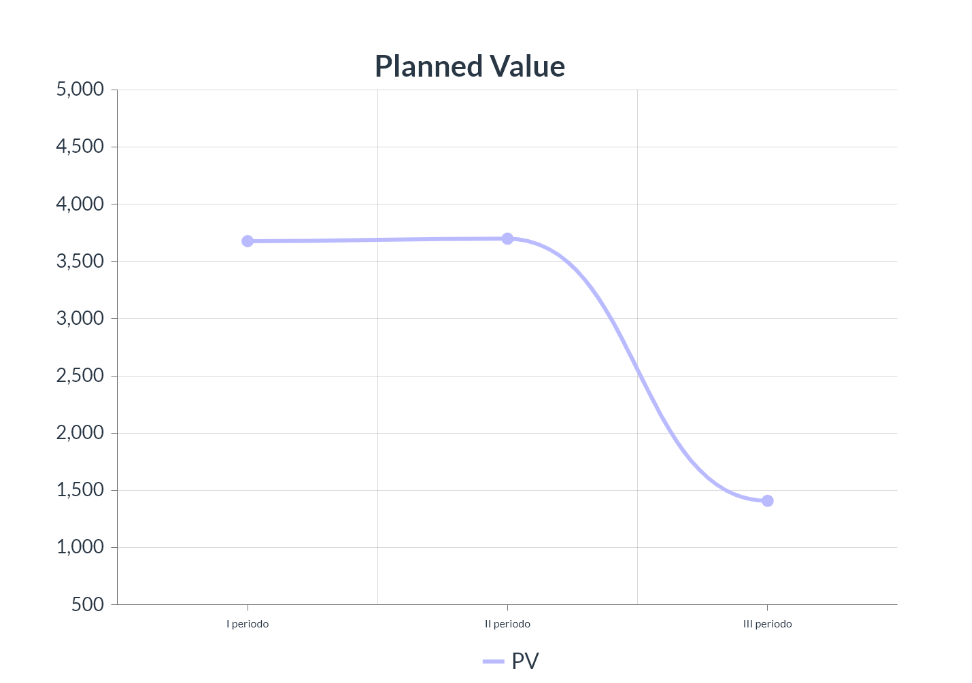
\includegraphics[width=10cm]{./res/images/PVGraph.png}
  \caption{Planned Value}
  \label{fig:Grafico Planned Value}
\end{figure}
\end{center}
\pagebreak
\paragraph{Actual Cost}
\begin{center}
\begin{figure}[H]
  \centering
  \renewcommand{\thefigure}{2}
  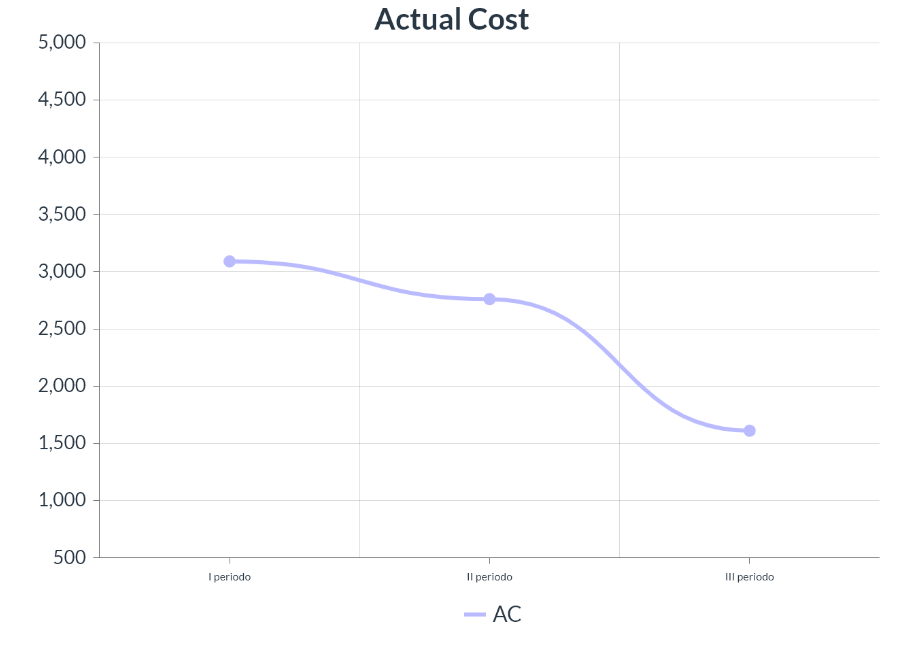
\includegraphics[width=10cm]{./res/images/ACGraph.png}
  \caption{Actual Cost}
  \label{fig:Grafico Actual Cost}
\end{figure}
\end{center}
\paragraph{Earned Value}
\begin{center}
\begin{figure}[H]
  \centering
  \renewcommand{\thefigure}{3}
  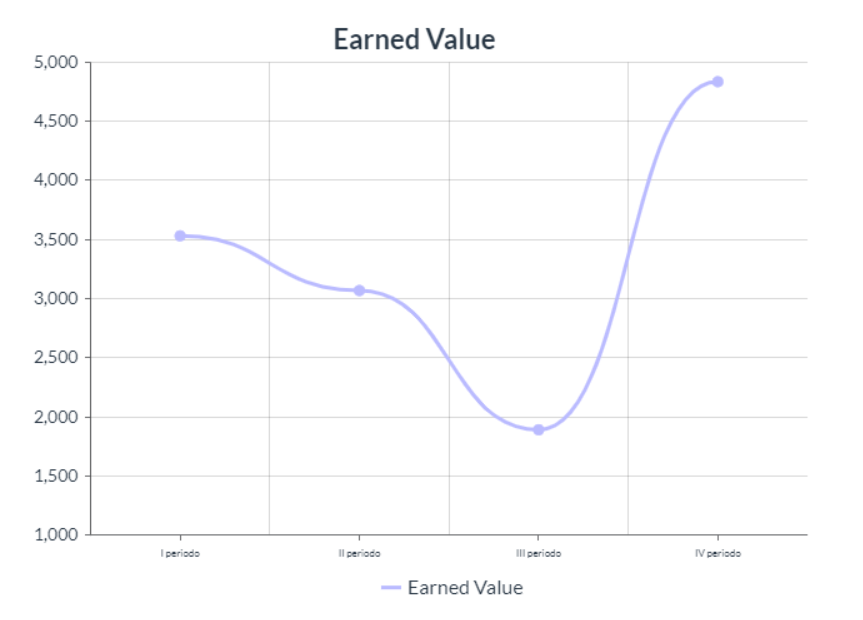
\includegraphics[width=10cm]{./res/images/EVGraph.png}
  \caption{Earned Value}
  \label{fig:Grafico Earned Value}
\end{figure}
\end{center}
\pagebreak
\paragraph{Cost Variance}
\begin{center}
\begin{figure}[H]
  \centering
  \renewcommand{\thefigure}{4}
  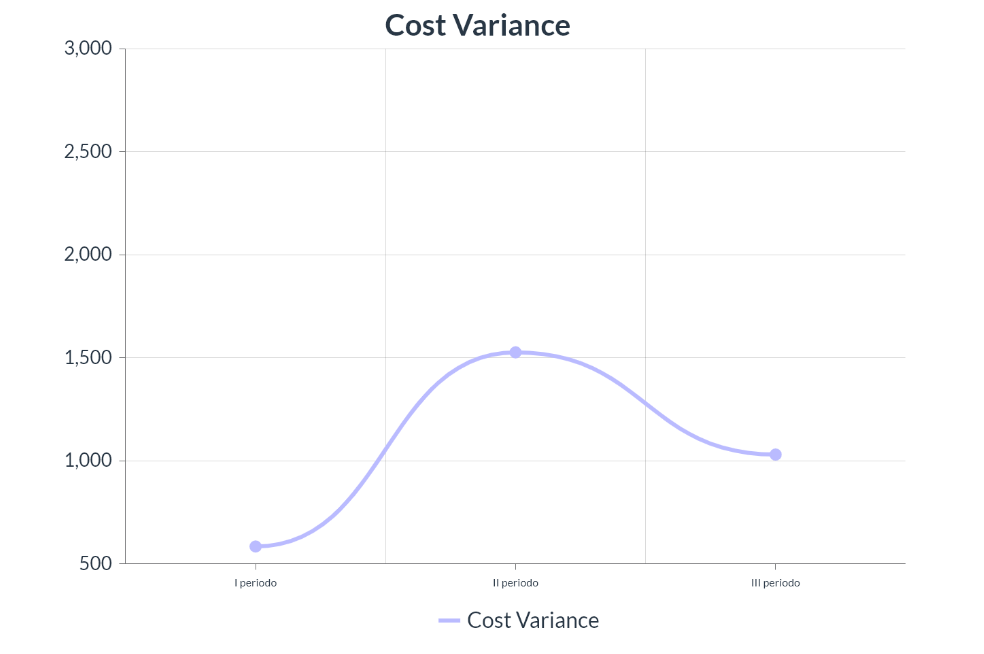
\includegraphics[width=10cm]{./res/images/CVGraph.png}
  \caption{Cost Variance}
  \label{fig:Grafico Cost Variance}
\end{figure}
\end{center}

\paragraph{Schedule Variance}
\begin{center}
\begin{figure}[H]
  \centering
  \renewcommand{\thefigure}{5}
  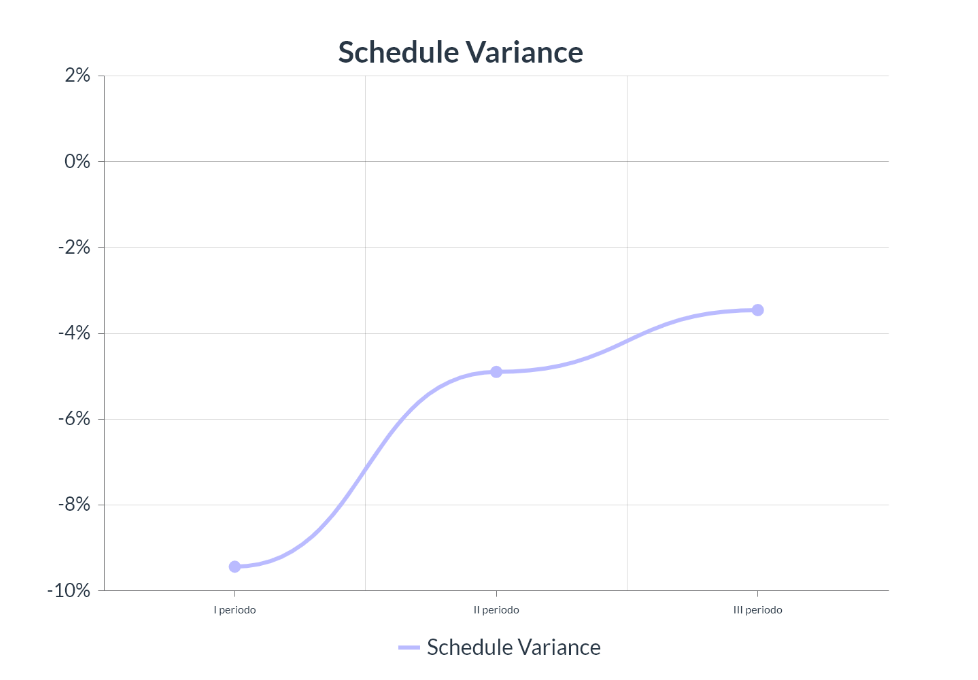
\includegraphics[width=10cm]{./res/images/SVGraph.png}
  \caption{Schedule Variance}
  \label{fig:Grafico Schedule Variance}
\end{figure}
\end{center}
\pagebreak
\paragraph{Budget Variance}
\begin{center}
\begin{figure}[H]
  \centering
  \renewcommand{\thefigure}{6}
  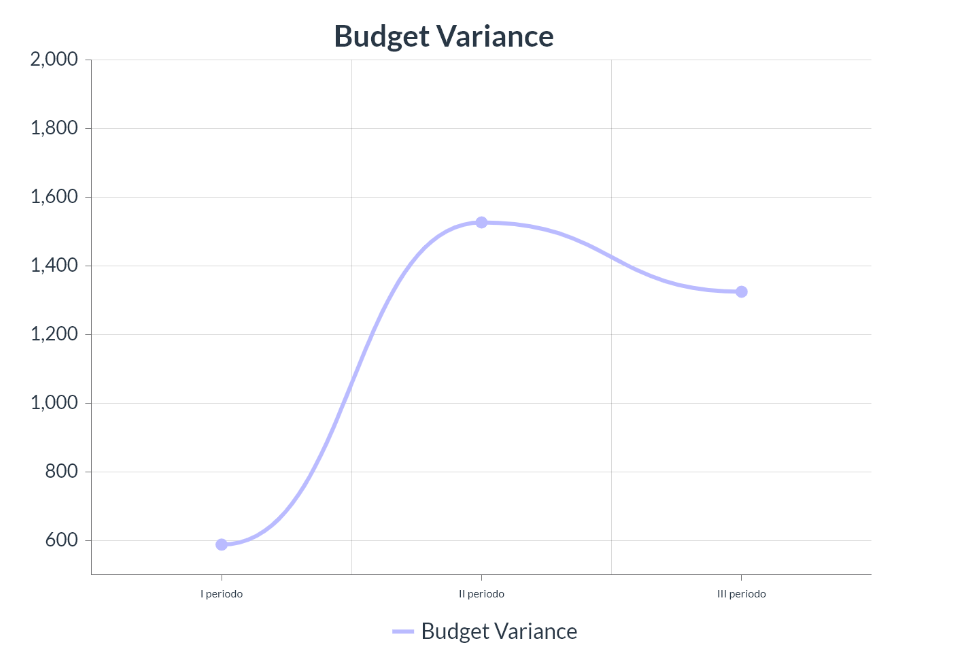
\includegraphics[width=10cm]{./res/images/BVGraph.png}
  \caption{Budget Variance}
  \label{fig:Grafico Budget Variance}
\end{figure}
\end{center}

\subsubsection{Indice di Gulpease}
\noindent Nella seguente tabella vengono riportati gli indici di Gulpease calcolati sulle ultime versioni dei seguenti documenti.\\
Per calcolare i seguenti valori non sono stati considerati: i changelog, la pagina di introduzione del documento, l'indice, tabelle con valori, intestazioni a piè di pagina, captions e la sezione di "Informazioni generali" nei verbali. Sono state incluse invece le colonne di tabelle contenenti descrizioni significative e gli elenchi puntati che contenevano frasi significative. 
\begin{longtable}{ 
		>{\centering}M{0.45\textwidth} 
		>{\centering}M{0.17\textwidth}
		>{\centering}M{0.25\textwidth} 
		}
	\rowcolorhead
	\headertitle{Documento} &
	\centering \headertitle{Valore} &	
	\headertitle{Esito} 
	\endfirsthead	
	\endhead
	
	\textit{Analisi dei Requisiti} & 80 & Superato\tabularnewline
	\textit{Glossario} & 72 & Superato\tabularnewline
	\textit{Norme di Progetto} & 74 & Superato\tabularnewline
	\textit{Piano di Progetto} & 63 & Superato\tabularnewline
	\textit{Piano di Qualifica} & 76 & Superato\tabularnewline
	\textit{Studio di Fattibilità} & 80 & Superato\tabularnewline
	VE 22-10-25 & 82 & Superato\tabularnewline
	VE 22-10-26 & 84 & Superato\tabularnewline
	VE 22-11-17	& 75 & Superato\tabularnewline
	VE 23-01-11	& 57 & Superato\tabularnewline
	VE 23-01-18	& 69 & Superato\tabularnewline
	VE 23-02-17 & 70 & Superato\tabularnewline
	VE 23-04-05 & 60 & Superato\tabularnewline
	VE 23-04-14 & 63 & Superato\tabularnewline
	VE 23-05-12 & 64 & Superato\tabularnewline
	VI 22-10-25 & 74 & Superato\tabularnewline
	VI 22-10-26 & 79 & Superato\tabularnewline
	VI 22-11-04 & 63 & Superato\tabularnewline
	VI 22-11-09 & 88 & Superato\tabularnewline
	VI 22-11-16 & 63 & Superato\tabularnewline
	VI 22-11-23 & 72 & Superato\tabularnewline
	VI 22-12-01 & 60 & Superato\tabularnewline
	VI 22-12-07 & 78 & Superato\tabularnewline
	VI 22-12-14 & 69 & Superato\tabularnewline
	VI 23-01-04 & 63 & Superato\tabularnewline
	VI 23-01-25 & 68 & Superato\tabularnewline
	VI 23-02-01 & 65 & Superato\tabularnewline
	VI 23-02-08 & 58 & Superato\tabularnewline
	VI 23-02-24 & 68 & Superato\tabularnewline
	VI 23-02-28 & 65 & Superato\tabularnewline
	VI 23-03-16 & 67 & Superato\tabularnewline
	VI 23-04-23 & 70 & Superato\tabularnewline
	VI 23-05-05 & 67 & Superato\tabularnewline
	
\end{longtable}

\begin{center}
\begin{figure}[H]
  \centering
  \renewcommand{\thefigure}{7}
  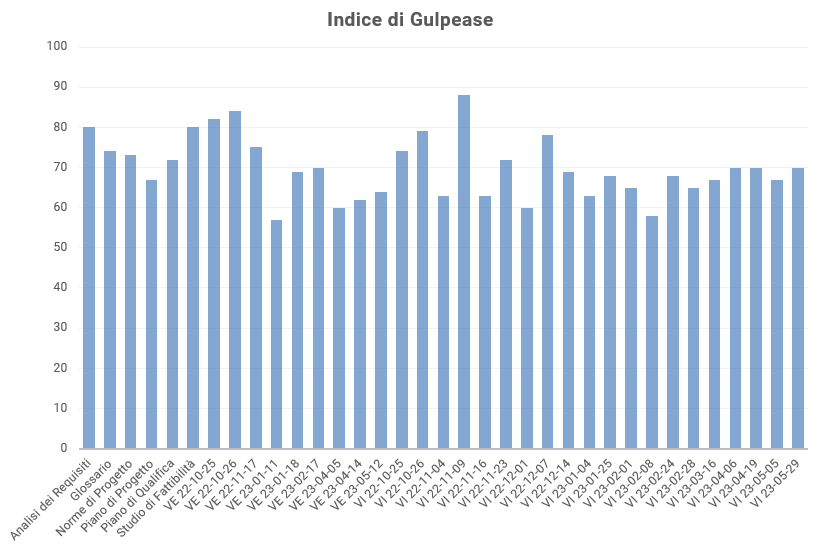
\includegraphics[width=10cm]{./res/images/GulpeaseGen.png}
  \caption{Indice di Gulpease dei documenti}
  \label{fig:Indice di Gulpease dei documenti}
\end{figure}
\end{center}
\pagebreak
\noindent Qui ora vengono riportati i grafici che analizzano l'andamento dell'indice di Gulpease di documenti in continua evoluzione.
\paragraph{Indice di Gulpease - \textit{Analisi dei Requisiti}}
\begin{center}
\begin{figure}[H]
  \centering
  \renewcommand{\thefigure}{8}
  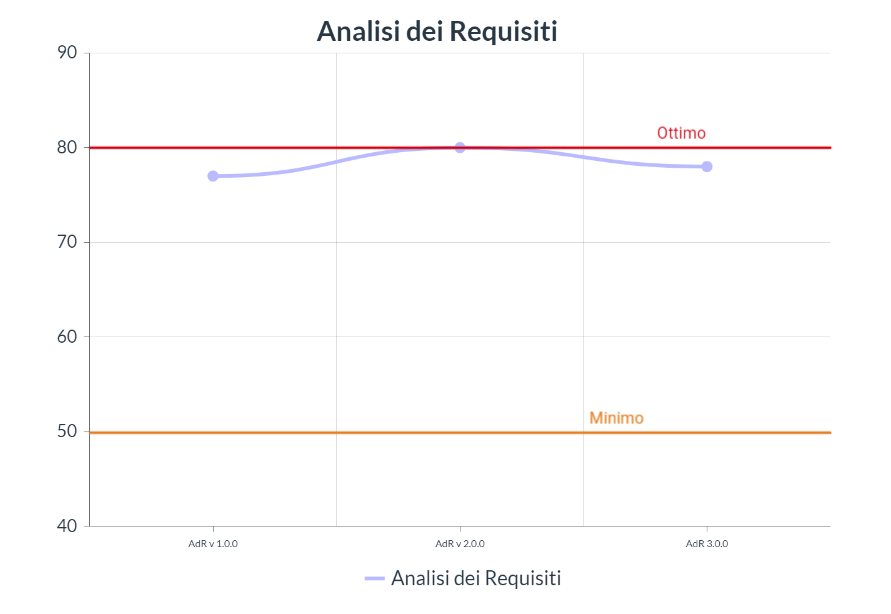
\includegraphics[width=10cm]{./res/images/AdRGraph.png}
  \caption{Indice di Gulpease - \textit{Analisi dei Requisiti}}
  \label{fig:Indice di Gulpease - Analisi dei Requisiti}
\end{figure}
\end{center}
\pagebreak
\paragraph{Indice di Gulpease - \textit{Norme di Progetto}}
\begin{center}
\begin{figure}[H]
  \centering
  \renewcommand{\thefigure}{9}
  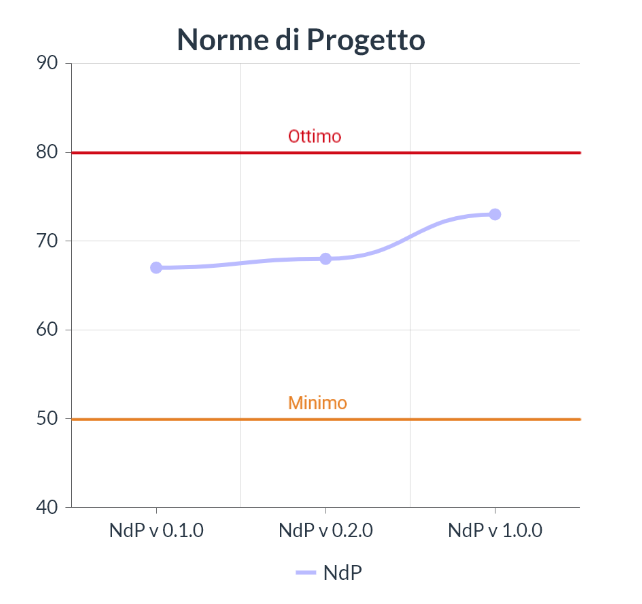
\includegraphics[width=10cm]{./res/images/NdPGraph.png}
  \caption{Indice di Gulpease - \textit{Norme di Progetto}}
  \label{fig:Indice di Gulpease - Norme di Progetto}
\end{figure}
\end{center}
\pagebreak
\paragraph{Indice di Gulpease - \textit{Piano di Progetto}}
\begin{center}
\begin{figure}[H]
  \centering
  \renewcommand{\thefigure}{10}
  \includegraphics[width=10cm]{./res/images/PdPGraph.png}
  \caption{Indice di Gulpease - \textit{Piano di Progetto}}
  \label{fig:Indice di Gulpease - Piano di Progetto}
\end{figure}
\end{center}
\pagebreak
\paragraph{Indice di Gulpease - \textit{Piano di Qualifica}}
\begin{center}
\begin{figure}[H]
  \centering
  \renewcommand{\thefigure}{11}
  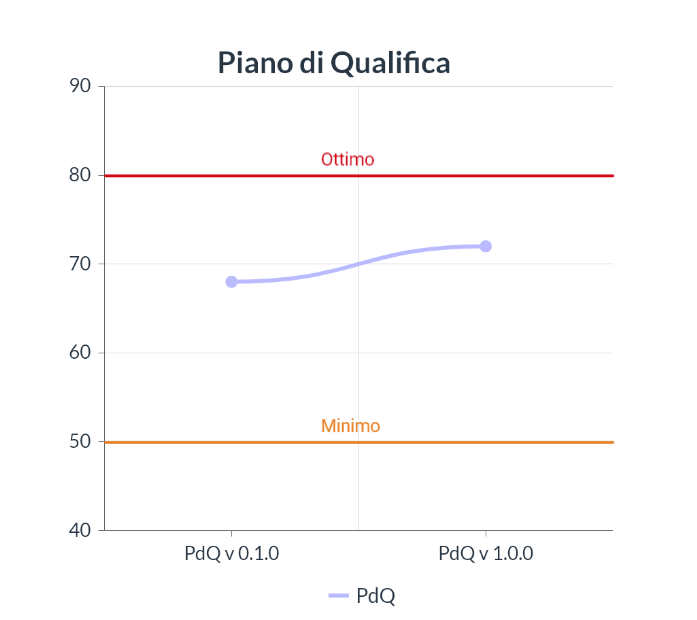
\includegraphics[width=10cm]{./res/images/PdQGraph.png}
  \caption{Indice di Gulpease - \textit{Piano di Qualifica}}
  \label{fig:Indice di Gulpease - Piano di Qualifica}
\end{figure}
\end{center}

\subsection{Verifica della qualità dei prodotti\textsubscript{g}}
In questa sezione vengono riportati i risultati dell'attività di verifica\textsubscript{g} effettuata relativa alla qualità del prodotto\textsubscript{g}, nel contesto del PoC\textsubscript{g}.\\
La metrica di Percentuale di requisiti soddisfatti non è stata testata in quanto non siamo ancora nella fase di Codifica.

\begin{longtable}{ 
		>{\centering}M{0.45\textwidth} 
		>{\centering}M{0.17\textwidth}
		>{\centering}M{0.25\textwidth} 
		}
	\rowcolorhead
	\headertitle{Metrica} &
	\centering \headertitle{Valore} &	
	\headertitle{Esito} 
	\endfirsthead	
	\endhead
	Percentuale di requisiti soddisfatti& - & Non testato\tabularnewline
	Densità di fallimenti durante l'esecuzione& 0\% & Superato\tabularnewline
	Tempo medio di risposta & minore di 1s & Superato\tabularnewline
	Tempo di caricamento& 7 secondi & Superato\tabularnewline
	Facilità di apprendimento& 90 secondi & Superato\tabularnewline
	Densità dei commenti & 15,93\% & Superato\tabularnewline
	Browser supportati & 100\% & Superato\tabularnewline
\end{longtable}
\noindent Nella seguente tabella è stata calcolata la Complessità Ciclomatica del PoC\textsubscript{g}.
\begin{longtable}{ 
		>{\centering}M{0.40\textwidth} 
		>{\centering}M{0.15\textwidth}
		>{\centering}M{0.20\textwidth}
		}
	\rowcolorhead
	\headertitle{Modulo} &
	\headertitle{Valore} &
	\headertitle{Esito} 	
	\endfirsthead	
	\endhead
	Player.js & 2 & Superato\tabularnewline
	Light.js & 1 & Superato\tabularnewline
	Product.js & 1 & Superato\tabularnewline
	Raycasting.js & 6 & Superato\tabularnewline
	Renderer.js & 2 & Superato\tabularnewline
	Showroom\_poc.js & 1 & Superato\tabularnewline
	Source\_loader.js & 2 & Superato\tabularnewline
	UI\_listeners.js & 1 & Superato\tabularnewline
	
\end{longtable}

Il PoC\textsubscript{g} è stato testato sui seguenti browser:
\begin{longtable}{ 
		>{\centering}M{0.45\textwidth} 
		>{\centering}M{0.25\textwidth} 
		}
	\rowcolorhead
	\headertitle{Browser} &
	\headertitle{Esito} 
	\endfirsthead	
	\endhead
	
	Google Chrome (versione $ \ge 110 $) & Supportato\tabularnewline
	Microsoft Edge (versione $ \ge 110 $) & Supportato\tabularnewline
	Mozilla Firefox (versione $ \ge 109 $) & Supportato\tabularnewline
	Safari (versione $ \ge 16 $) & Supportato\tabularnewline
	Opera (versione $ \ge 95 $) & Supportato\tabularnewline

\end{longtable}

\section{Specifica dei Test}
\begin{itemize}
\item Test di unità: vengono stabiliti durante la progettazione e servono per verificare le singole unità software;
\item Test di integrazione: vengono stabiliti durante la progettazione e servono per integrare il funzionamento di più unità;
\item Test di accettazione: vengono effettuati insieme al proponente\textsubscript{g} durante la fase di collaudo;
\item Test di sistema: vengono stabiliti durante l'\textit{Analisi dei Requisiti} e servono per accertare la copertura dei requisiti software definiti nel documento di \textit{Analisi dei Requisiti}.
\end{itemize}
Gli acronimi utilizzati in questo documento per identificare i test sono specificati dettagliatamente nel documento di \textit{Norme di Progetto}.
In questa sezione vengono utilizzate le seguenti sigle per lo stato di ogni test:
\begin{itemize}
\item \textbf{S}: test superato
\item \textbf{N}: test non implementato
\end{itemize}

\subsection{Test di unità}
Per garantire il funzionamento dei singoli componenti che possono lavorare in maniera autonoma senza bisogno di dipendenze abbiamo effettuato questi test. Non abbiamo ritenuto necessario testare componenti o parti di componenti che:
\begin{itemize}
	\item Utilizzavano funzionalità già assodate e documentate;
	\item Componenti che raggruppavano altri componenti.
\end{itemize} 
\begin{longtable}{
		>{\centering}M{0.20\textwidth}
		>{\centering}M{0.35\textwidth}	 
		>{\centering}M{0.20\textwidth} 
		}
	\rowcolorhead
	\headertitle{Test} &
	\centering \headertitle{Descrizione} &	
	\headertitle{Stato} 
	\endfirsthead	
	\endhead
TU1 & Si verifichi che la posizione del player cambi quando utilizza i tasti di movimento & S\tabularnewline
TU2 & Si verifichi che la rotazione del player cambi quando muove la visuale col mouse & S\tabularnewline
TU3 & Si verifichi che avvenga il cambiamento colore ad un oggetto interagibile & S\tabularnewline
TU4 & Si verifichi la funzionalità dell’aggiunta all’array che rappresenta gli oggetti nel carrello e l’incremento del costo totale & S\tabularnewline
TU5 & Si verifichi che la funzionalità di aggiungere un oggetto al carrello funzioni solo con oggetti validi & S\tabularnewline
TU6 & Si verifichi la possibilità di utilizzare i selettori Redux per reperire l’array logico del carrello e il costo totale & S\tabularnewline
TU7 & Si verifichi la funzionalità della rimozione totale dall’array del carrello & S\tabularnewline
TU8 & Si verifichi che la funzionalità di rimozione totale dell’array carrello funzioni anche se il carrello è vuoto & S\tabularnewline
TU9 & Si verifichi la funzionalità di eliminazione singola dal carrello & S\tabularnewline
TU10 & Si verifichi che l’eliminazione singola funziona solo con oggetti realmente presenti nell’array carrello & S\tabularnewline
TU11 & Si verifichi che il raycaster funzioni & S\tabularnewline
TU12 & Si verifichi che funzioni la possibilità di aggiungere quantità di un oggetto selezionato & S\tabularnewline
TU13 & Si verifichi che funzioni la possibilità di diminuire quantità di un oggetto selezionato & S\tabularnewline
\end{longtable}

\subsection{Test di integrazione}
Per assicurare che ogni componente lavori correttamente con gli altri componenti, il gruppo ha deciso di effettuare i seguenti Test di Integrazione.
\begin{longtable}{
		>{\centering}M{0.20\textwidth}
		>{\centering}M{0.35\textwidth}	 
		>{\centering}M{0.20\textwidth} 
		}
	\rowcolorhead
	\headertitle{Test} &
	\centering \headertitle{Descrizione} &	
	\headertitle{Stato} 
	\endfirsthead	
	\endhead
TI1 & Si verifichi che la modifica di cambiamento colore venga apportata ad un oggetto esempio nel file JSON contenente i prodotti interagibili & S\tabularnewline
TI2 & Si verifichi che un elemento nel carrello , se eliminato singolarmente, scompaia dal componente Cart e anche dall’array logico del carrello & S\tabularnewline
TI3 & Si verifichi che il bottone “Remove all” funzioni rimuovendo sia da Cart che da cartSlice tutti gli oggetti & S\tabularnewline
TI4 & Si verifichi che il bottone “Remove all” funzioni anche se il carrello è vuoto & S\tabularnewline
TI5 & Si verifichi che il cambio di colore nella Sidebar venga salvato & S\tabularnewline
TI6 & Si verifichi che il colore ritorni a standard se viene deselezionata una modifica di colore & S\tabularnewline
TI7 & Si verifichi che venga aggiunto un oggetto al carrello dalla sidebar & S\tabularnewline
TI8 & Si verifichi che venga aggiunta la quantità selezionata di un oggetto già presente nel carrello & S\tabularnewline
\end{longtable}
\subsection{Test di accettazione}
Questi test verranno stabiliti durante la fase di Collaudo.

\subsection{Test di sistema}
Per assicurare che vengano rispettati i requisiti concordati nel documento di \textit{Analisi dei Requisiti}, vengono eseguiti i seguenti test di sistema.
\begin{longtable}{
		>{\centering}M{0.20\textwidth}
		>{\centering}M{0.35\textwidth}	 
		>{\centering}M{0.20\textwidth} 
		}
	\rowcolorhead
	\headertitle{Test} &
	\centering \headertitle{Descrizione} &	
	\headertitle{Stato} 
	\endfirsthead	
	\endhead
TSRF1 & Si verifica\textsubscript{g} che l'utente possa aggiungere, l'oggetto con cui sta interagendo, nel carrello & S \tabularnewline
TSRF2 & Si verifica\textsubscript{g} che l'utente possa visualizzare il contenuto del carrello & S \tabularnewline
TSRF2.1 & Si verifica\textsubscript{g} che l'utente possa visualizzare la lista degli oggetti presenti nel carrello & S \tabularnewline
TSRF2.1.1 & Si verifica\textsubscript{g} che l'utente possa interagire con un oggetto nel carrello & S \tabularnewline
TSRF2.1.1.1 & Si verifica\textsubscript{g} che l'utente possa visualizzare la caratteristica del nome di ogni oggetto presente nella lista degli oggetti presenti nel carrello & S \tabularnewline
TSRF2.1.1.2 & Si verifica\textsubscript{g} che l'utente possa visualizzare la caratteristica del costo di ogni oggetto presente nella lista degli oggetti presenti nel carrello & S \tabularnewline
TSRF2.1.1.3 & Si verifica\textsubscript{g} che l'utente possa visualizzare la caratteristica della quantità di ogni oggetto presente nella lista degli oggetti presenti nel carrello & S \tabularnewline
TSRF2.2 & Si verifica\textsubscript{g} che l'utente possa visualizzare il costo totale degli oggetti che ha inserito nel carrello & S \tabularnewline
TSRF3 & Si verifica\textsubscript{g} che l'utente abbia la possibilità di rimuovere tutti gli oggetti dal carrello & S \tabularnewline
TSRF4 & Si verifica\textsubscript{g} che l'utente abbia la possibilità di rimuovere un singolo oggetto dal carrello & S \tabularnewline
TSRF5 & Si verifica\textsubscript{g} che l'utente possa muoversi in maniera direzionale & S \tabularnewline
TSRF5.1 & Si verifica\textsubscript{g} che l'utente possa compiere movimenti direzionali nell'asse X & S \tabularnewline
TSRF5.2 & Si verifica\textsubscript{g} che l'utente possa compiere movimenti direzionali nell'asse Y & S \tabularnewline
TSRF5.3 & Si verifica\textsubscript{g} che l'utente possa compiere movimenti direzionali nell'asse Z & S \tabularnewline
TSRF6 & Si verifica\textsubscript{g} che l'utente possa compiere spostamenti di camera & S \tabularnewline
TSRF6.1 & Si verifica\textsubscript{g} che l'utente possa compiere spostamenti di camera nell'asse X & S \tabularnewline
TSRF6.2 & Si verifica\textsubscript{g} che l'utente possa compiere spostamenti di camera nell'asse Y & S \tabularnewline
TSRF7 & Si verifica\textsubscript{g} che l'utente possa modificare la combinazione dei colori di un oggetto & S \tabularnewline
TSRF8 & Si verifica\textsubscript{g} che l'utente venga notificato in caso non fosse possibile modificare un oggetto & S \tabularnewline
TSRF9 & Si verifica\textsubscript{g} che l'utente possa visualizzare la lista degli oggetti della stanza in cui si trova & N \tabularnewline
TSRF9.1 & Si verifica\textsubscript{g} che l'utente possa visualizzare un singolo oggetto nella lista degli oggetti della stanza in cui si trova & N \tabularnewline
TSRF9.1.1 & Si verifica\textsubscript{g} che l'utente possa visualizzare la caratteristica del nome di ogni oggetto della lista degli oggetti della stanza in cui si trova & N \tabularnewline
TSRF10 & Si verifica\textsubscript{g} che l'utente possa visualizzare tutti i dettagli di un oggetto selezionato & S \tabularnewline
TSRF11 & Si verifica\textsubscript{g} che l'utente abbia la possibilità di riposizionarsi vicino ad un oggetto nella stanza in cui si trova & N \tabularnewline
TSRF12 & Si verifica\textsubscript{g} che l'utente possa riposizionarsi in una stanza da lui selezionata & N \tabularnewline
TSRF13 & Si verifica\textsubscript{g} che l'utente venga notificato in caso il riposizionamento in una stanza non sia possibile & N \tabularnewline
TSRF14 & Si verifica\textsubscript{g} che l'utente venga notificato in caso il riposizionamento in prossimità di un oggetto selezionato non sia concesso & N \tabularnewline
TSRF15 & Si verifica\textsubscript{g} che l'utente possa visualizzare la lista delle stanze & N \tabularnewline
TSRF15.1 & Si verifica\textsubscript{g} che l'utente possa visualizzare una singola stanza dalla lista delle stanze & N \tabularnewline
TSRF15.1.1 & Si verifica\textsubscript{g} che l'utente possa visualizzare la caratteristica del nome di ogni stanza dalla lista delle stanze & N \tabularnewline
TSRF15.1.2 & Si verifica\textsubscript{g} che l'utente possa visualizzare la caratteristica della tipologia di oggetti presenti in ogni stanza nella lista delle stanze & N \tabularnewline
TSRF16 & Si verifica\textsubscript{g} che l'utente possa riposizionare un oggetto presente nella stanza in cui si trova & N \tabularnewline
TSRF17 & Si verifica\textsubscript{g} che l'utente non possa riposizionare un oggetto in una coordinata non legittima & N \tabularnewline
TSRF18 & Si verifica\textsubscript{g} che l'utente sia in grado ad illuminare l'ambiente davanti a lui & S \tabularnewline
TSRF19 & Si verifica\textsubscript{g} che l'utente venga notificato se il contenuto del carrello è vuoto & S \tabularnewline
TSRF20 & Si verifica\textsubscript{g} che l'utente possa visualizzare un oggetto illuminato & S \tabularnewline
\end{longtable}

\subsection{Tracciamento dei test}
\subsubsection{Test di Sistema - Requisiti}
\begin{longtable}{
		>{\centering}M{0.25\textwidth}
		>{\centering}M{0.25\textwidth}	 
		}
	\rowcolorhead
	\headertitle{Test di sistema} &
	\headertitle{Requisiti}
	\endfirsthead	
	\endhead
TSRF1 & RF1\tabularnewline
TSRF2 & RF2\tabularnewline
TSRF2.1 & RF2.1\tabularnewline
TSRF2.1.1 & RF2.1.1\tabularnewline
TSRF2.1.1.1 & RF2.1.1.1\tabularnewline
TSRF2.1.1.2 & RF2.1.1.2\tabularnewline
TSRF2.1.1.3 & RF2.1.1.3\tabularnewline
TSRF2.2 & RF2.2\tabularnewline
TSRF3 & RF3\tabularnewline
TSRF4 & RF4\tabularnewline
TSRF5 & RF5\tabularnewline
TSRF5.1 & RF5.1\tabularnewline
TSRF5.2 & RF5.2\tabularnewline
TSRF5.3 & RF5.3\tabularnewline
TSRF6 & RF6\tabularnewline
TSRF7 & RF7\tabularnewline
TSRF8 & RF8\tabularnewline
TSRF9 & RF9\tabularnewline
TSRF9.1 & RF9.1\tabularnewline
TSRF9.1.1 & RF9.1.1\tabularnewline
TSRF10 & RF10\tabularnewline
TSRF11 & RF11\tabularnewline
TSRF12 & RF12\tabularnewline
TSRF13 & RF13\tabularnewline
TSRF14 & RF14\tabularnewline
TSRF15 & RF15\tabularnewline
TSRF15.1 & RF5.1\tabularnewline
TSRF15.1.1 & RF15.1.1\tabularnewline
TSRF15.1.2 & RF15.1.2\tabularnewline
TSRF16 & RF16\tabularnewline
TSRF17 & RF17\tabularnewline
TSRF18 & RF18\tabularnewline
TSRF19 & RF19\tabularnewline
TSRF20 & RF20\tabularnewline

\end{longtable}

\subsubsection{Test di Unità - File di Test}
\begin{longtable}{
		>{\centering}M{0.10\textwidth}
		>{\centering}M{0.30\textwidth}
		>{\centering}M{0.45\textwidth}	 
		}
	\rowcolorhead
	\headertitle{Test} &
	\centering \headertitle{File di test} &	
	\centering \headertitle{Nome test} 
	\endfirsthead	
	\endhead
TU1 & \_\_test\_\_/playerSlice.test.js & it(’should set the player position’)\{ … \}\tabularnewline
TU2 & \_\_test\_\_/playerSlice.test.js & it(’should set the player rotation’)\{ … \}\tabularnewline
TU3 & \_\_test\_\_/productSlice.test.js & it('Should change color to the product in example')\{ … \}\tabularnewline
TU4 & \_\_test\_\_/cartSlice.test.js & it('Should add an item to the array (that represents the logic of the cart) of the slice and increment the totalCost’)\{ … \}\tabularnewline
TU5 & \_\_test\_\_/cartSlice.test.js & it('Should not be able to add this item’) \{ … \}\tabularnewline
TU6 & \_\_test\_\_/cartSlice.test.js & it('Should be able to use the cartItems selector and the totalCost selector’)\{ … \}\tabularnewline
TU7 & \_\_test\_\_/cartSlice.test.js & it('Should remove all the item in the cart')\{ … \}\tabularnewline
TU8 & \_\_test\_\_/cartSlice.test.js & it('Should remove all the items even if the cart is empty’)\{ … \}\tabularnewline
TU9 & \_\_test\_\_/cartSlice.test.js & it('Should remove the item in example’)\{ … \}\tabularnewline
TU10 & \_\_test\_\_/cartSlice.test.js & it('Should be able to work even if the item provided do not exist in the cart’)\{ … \}\tabularnewline
TU11 & \_\_test\_\_/useRaycasterLogic.test.js & it('should update intersects when mouse moves’)\{ … \}\tabularnewline
TU12 & \_\_test\_\_/productSidebar.test.js & it('Should add more then one quantity of the item selected’)\{ … \}\tabularnewline
TU13 & \_\_test\_\_/productSidebar.test.js & it('Should decrease of one the quantity of the item’)\{ … \}\tabularnewline
\end{longtable}

\subsubsection{Test di Integrità - File di Test}
\begin{longtable}{
		>{\centering}M{0.10\textwidth}
		>{\centering}M{0.30\textwidth}
		>{\centering}M{0.45\textwidth}	 
		}
	\rowcolorhead
	\headertitle{Test} &
	\centering \headertitle{File di test} &	
	\centering \headertitle{Nome test} 
	\endfirsthead	
	\endhead
TI1 & \_\_test\_\_/productSlice.test.js & it('Should change color to the product with the ID=1 imported from the JSON file’)\{ … \} \tabularnewline
TI2 & \_\_test\_\_/cart.test.js & it('Should stop rendering item in cart when clicking "X" button’)\{ … \}\tabularnewline
TI3 & \_\_test\_\_/cart.test.js & it('Should stop rendering all items in cart when clicking "Remove all" button’)\{ … \}\tabularnewline
TI4 & \_\_test\_\_/cart.test.js & it('Should try to remove the items and work even if cart is empty’)\{ … \}\tabularnewline
TI5	& \_\_test\_\_/productSidebar.test.js & it('Should change the variable selectedColor to the product in example’)\{ … \}\tabularnewline
TI6 & \_\_test\_\_/productSidebar.test.js & it('Should remove the selected color if the button with the current color is pressed, putting the standard color to the item’)\{ … \}\tabularnewline
TI7 & \_\_test\_\_/productSidebar.test.js & it('Should add an item to the cart’)\{ … \}\tabularnewline
TI8 & \_\_test\_\_/productSidebar.test.js & it('Should add more than one quantity of the item to the cart, testing also if it adds the quantity to the item that is already in the cart’)\{ … \}\tabularnewline
\end{longtable}
\pagebreak

\end{document}

\subsubsection{\textit{Glossario}}
All'interno del documento si possono trovare dei termini che possono risultare ambigui a seconda del contesto, o non conosciuti dagli utilizzatori.\\\
Per ovviare ad errori di incomprensione che possono portare a problemi di vario genere e rallentamenti si è deciso di stilare un elenco di termini 
di interesse accompagnati da una descrizione dettagliata del loro significato.\\
I termini presenti all'interno del \textit{Glossario} vengono indicati con il pedice 'g' come nell'esempio seguente: termine\textsubscript{g}.
Il \textit{Glossario} ordina i termini in ordine alfabetico in modo da permetterne una facile e veloce ricerca.
Ogni componente del gruppo all'inserimento di un termine ritenuto ambiguo deve preoccuparsi di aggiornare il \textit{Glossario} in modo da mantenerlo sempre aggiornato.
